\section{Experiments}
This appendix contains all of the included experiments from which we have derived our results. Each of the plots, depending on the number of experiments, will depict the mean scores of the experiments or the experiments themselves.\\
With each experiment, a table detailing the parameter values will be included for others who would want to reproduce these experiments. Depending on the optimizer (weather it is Cross Entropy or CMA), the table will contain some custom rows, unique for the specific algorithm.\\
Similar for all experiments is the 30 games played with the new mean of each generation to generate the learning curve.\\
The tables are formatted 
\begin{table}[h]
\centering
\caption{Overview of the two table formats}
\begin{tabular}{l r}
Optimizer & CMA\\
Number of Evaluations & -\\
Number of Learning Games & -\\
Population size& -\\
Parent size & -\\
Games per Agent & -\\
Tetris Type & -\\
\hline
Recombination Type & -\\
Initial Sigma & -\\
 & \\
\end{tabular}
\quad
\begin{tabular}{l r}
Optimizer & Cross Entropy\\
Number of Evaluations & -\\
Number of Learning Games & -\\
Population size & -\\
Parent size & -\\
Games per Agent & -\\
Tetris Type & -\\
\hline
Sigma & -\\
Noise Type & -\\
Noise & -
\end{tabular}
\end{table}

\clearpage

\subsection{Game Complexity}
Experiments to test if game complexity can be used for tuning the CMA and CE configurations.

\begin{table}[h]
\centering
\caption{Cross Entropy settings for testing game complexity}
\begin{tabular}{l r}
Optimizer & Cross Entropy\\
Number of Evaluations & 8000\\
Population size & 100\\
Parent size & 10\\
Games per Agent & 1\\
Tetris Type & Hard\\
\hline
Sigma & 100\\
Noise Type & No noise\\
Noise & -
\end{tabular}
\quad
\begin{tabular}{l r}
Optimizer & Cross Entropy\\
Number of Evaluations & 8000\\
Population size & 100\\
Parent size & 10\\
Games per Agent & 1\\
Tetris Type & Normal\\
\hline
Sigma & 100\\
Noise Type & No noise\\
Noise & -
\end{tabular}
\end{table}

\begin{table}[h]
\centering
\caption{CMA settings for testing game complexity}
\begin{tabular}{l r}
Optimizer & CMA\\
Number of Evaluations & 8000\\
Number of Learning Games & 30\\
Population size& 13\\
Parent size & 6\\
Games per Agent & 1\\
Tetris Type & Hard\\
\hline
Recombination Type & Superlinear\\
Initial Sigma & 1
\end{tabular}
\quad
\begin{tabular}{l r}
Optimizer & CMA\\
Number of Evaluations & 8000\\
Number of Learning Games & 30\\
Population size& 13\\
Parent size & 6\\
Games per Agent & 1\\
Tetris Type & Normal\\
\hline
Recombination Type & Superlinear\\
Initial Sigma & 1
\end{tabular}
\end{table}



\clearpage

\subsection{Verification of Cross Entropy}
Using the same configuration as in "reference paper", we will reproduce the experiments to verify our implementation of Cross Entropy into the Shark Library.\\
\\
\begin{table}[h!]
\centering
\begin{tabular}{l r}
Optimizer & Cross Entropy\\
Number of Evaluations & 8000\\
Population size & 100\\
Parent size & 10\\
Games per Agent & 1\\
Tetris Type & Normal\\
\hline
Sigma & 100\\
Noise Type & No noise\\
Noise & -
\end{tabular}
\caption{Cross Entropy - No noise}
\end{table}

\begin{table}[h!]
\centering
\begin{tabular}{l r}
Optimizer & Cross Entropy\\
Number of Evaluations & 8000\\
Population size & 100\\
Parent size & 10\\
Games per Agent & 1\\
Tetris Type & Normal\\
\hline
Sigma & 100\\
Noise Type & Constant\\
Noise & 4
\end{tabular}
\caption{Cross Entropy - Constant noise}
\end{table}

\begin{table}[h!]
\centering
\begin{tabular}{l r}
Optimizer & Cross Entropy\\
Number of Evaluations & 8000\\
Population size & 100\\
Parent size & 10\\
Games per Agent & 1\\
Tetris Type & Normal\\
\hline
Sigma & 100\\
Noise Type & Linear decreasing\\
Noise & $max \left( 5 - \frac{t}{10}, 0 \right)$
\end{tabular}
\caption{Cross Entropy - Linear decreasing noise}
\end{table}


\clearpage

\subsection{Population and selection size}
We want to investigate if there exists a better configuration than the 100/10 which was also previously used by other researchers.\\
In Cross Entropy for the Tetris problem, 10 \% Parent selection is used as standard. However, we will also test 50 \% Parent selection is a configuration from CMA which we will also test.\\
The general testing parameters are as follows
\begin{table}[h]
\centering
\caption{General setup for Population/Parent size}
\begin{tabular}{l r}
Optimizer & Cross Entropy\\
Number of Evaluations & 8000\\
Population size & See table \ref{CEPopulationParentSize}\\
Parent size & See table \ref{CEPopulationParentSize}\\
Games per Agent & 1\\
Tetris Type & Normal\\
\hline
Sigma & 100\\
Noise Type & Constant\\
Noise & 4
\end{tabular}
\end{table}

with the following population/Parent size

\begin{table}[h]
\centering
\begin{tabular}{l l}
Population size & Parent size\\
\hline
12 & 1\\
12 & 3\\
12 & 5\\
22 & 2\\
22 & 5\\
22 & 11\\
50 & 5\\
50 & 12\\
50 & 25\\
100 & 10\\
100 & 25\\
100 & 50\\
200 & 20\\
200 & 50\\
200 & 100
\end{tabular}
\caption{Population/Parent size \label{CEPopulationParentSize}}
\end{table}

INSERT PLOTS HERE.\\
\\
quantile table and two graphs over the mean plots of 10 \% and 50 \% Parent size

\clearpage

\begin{figure}[H]
\centering
\begin{tabular}{r r | r r r r}
population & offspring & mean & Q1 & Q2 & Q3\\
\hline
12 & $10\%$  & 1585,3     & 93,0      & 113,5        & 220,7\\
12 & $25\%$  & 30.496,9   & 15.222,1  & 20.264,2     & 39.019,8\\
12 & $50\%$  & 39.824,2   & 26.457,0  & 33.663,4     & 49.743,7\\
22 & $10\%$  & 35.841,6   & 20.391,9  & 42.045,5     & 48.464,6\\
22 & $25\%$  & 80.884,9   & 56.042,5  & 71.900,2     & 78.653,4\\
22 & $50\%$  & 52.887,4   & 23.531,9  & 42.161,0     & 83.144,1\\
50 & $10\%$  & 95,623,1   & 82.738,9  & 93.388,9     & 111.351,5\\
50 & $25\%$  & 110.525,0  & 103.128,1 & 111.195,5    & 121.974,4\\
50 & $50\%$  & 69.130,7   & 52.511,0  & 64.351,6     & 91.488,6\\
100 & $10\%$ & 115.868,7  & 84.368,5  & 122.238,5    & 146.457,0\\
100 & $25\%$ & 70.011,1   & 58.008,0  & 69.588,2     & 80.432,7\\
100 & $50\%$ & 22.910,4   & 4.037,7   & 14.353,7     & 47.215,9\\
200 & $10\%$ & 85.181,7   & 45.201,5  & 96.803,1     & 117.578,0\\
200 & $25\%$ & 32.894,6   & 8688,7    & 25.333,1     & 58.434,8\\
200 & $50\%$ & 946,4      & 585,0     & 802,5        & 1.267,7
\end{tabular}
\caption{Cross Entropy configuration test, 
see Appendix for the full plots 
of the experiments.  \label{CEConfigTest}}
\end{figure}


\clearpage

\subsection{Optimal settings for Cross Entropy - Games per agent \label{appendixCEPopulationParent}}
Experiment to determine the optimal number of games played per agent for best resulting score at lowest evaluation cost.

\begin{table}[h]
\centering
\caption{General setup for Population/Parent size}
\begin{tabular}{l r}
Optimizer & Cross Entropy\\
Number of Evaluations & 80000\\
Population size & See table \ref{GamesPerAgentCE}\\
Parent size & See table \ref{GamesPerAgentCE}\\
Games per Agent & See table \ref{GamesPerAgentCE}\\
Tetris Type & Hard\\
\hline
Sigma & 100\\
Noise Type & Constant\\
Noise & 4
\end{tabular}
\end{table}

with the following population/Parent size and number of games played per agent


\begin{table}[H]
\centering
\begin{tabular}{c c c}
Population Size & Parent size & Games per Agent\\
\hline
$12$ & $10\%$ & 1/3/5/7/10\\
$12$ & $25\%$ & 1/3/5/7/10\\
$12$ & $50\%$ & 1/3/5/7/10\\
$22$ & $10\%$ & 1/3/5/7/10\\
$22$ & $25\%$ & 1/3/5/7/10\\
$22$ & $50\%$ & 1/3/5/7/10\\
$50$ & $10\%$ & 1/3/5/7/10\\
$50$ & $25\%$ & 1/3/5/7/10\\
$50$ & $50\%$ & 1/3/5/7/10\\
$100$ & $10\%$ & 1/3/5/7/10\\
$100$ & $25\%$ & 1/3/5/7/10\\
$100$ & $50\%$ & 1/3/5/7/10\\
$200$ & $10\%$ & 1/3/5/7/10\\
$200$ & $25\%$ & 1/3/5/7/10\\
$200$ & $50\%$ & 1/3/5/7/10
\end{tabular}
\caption{Games per agent CE experiment setup\label{GamesPerAgentCE}}
\end{table}

\clearpage

\begin{figure}
	\centering
	\captionsetup[subfigure]{justification=centering}
    \begin{subfigure}[b]{0.49\textwidth}
    	\caption{Population size 12, Parent size 1}
        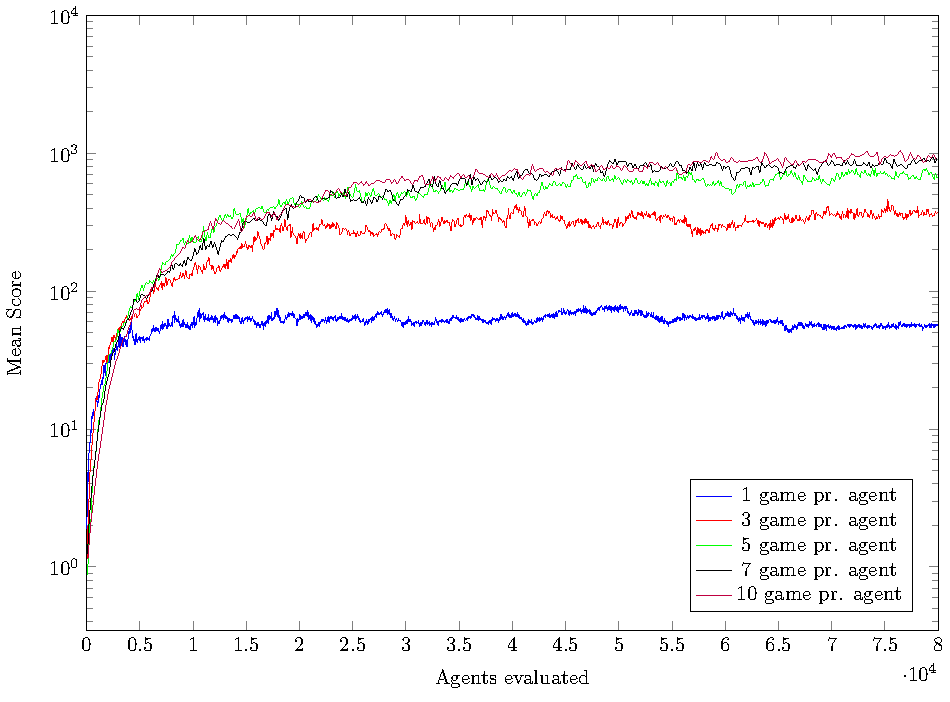
\includegraphics[width=\textwidth]{data/ce_population_offspring/12x_split/constant_l12_o1/mean/PlotFile.pdf}
    \end{subfigure} 
    \begin{subfigure}[b]{0.49\textwidth}
    	\caption{Population size 12, Parent size 3}
        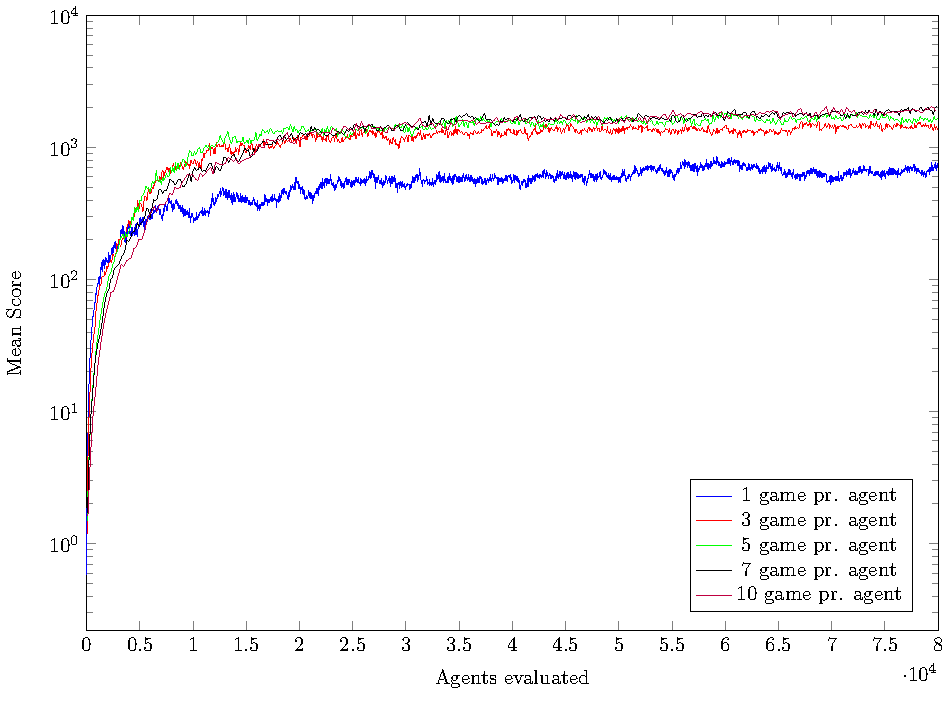
\includegraphics[width=\textwidth]{data/ce_population_offspring/12x_split/constant_l12_o3/mean/PlotFile.pdf}
    \end{subfigure}
    \begin{subfigure}[b]{0.49\textwidth}
    	\caption{Population size 12, Parent size 6}
        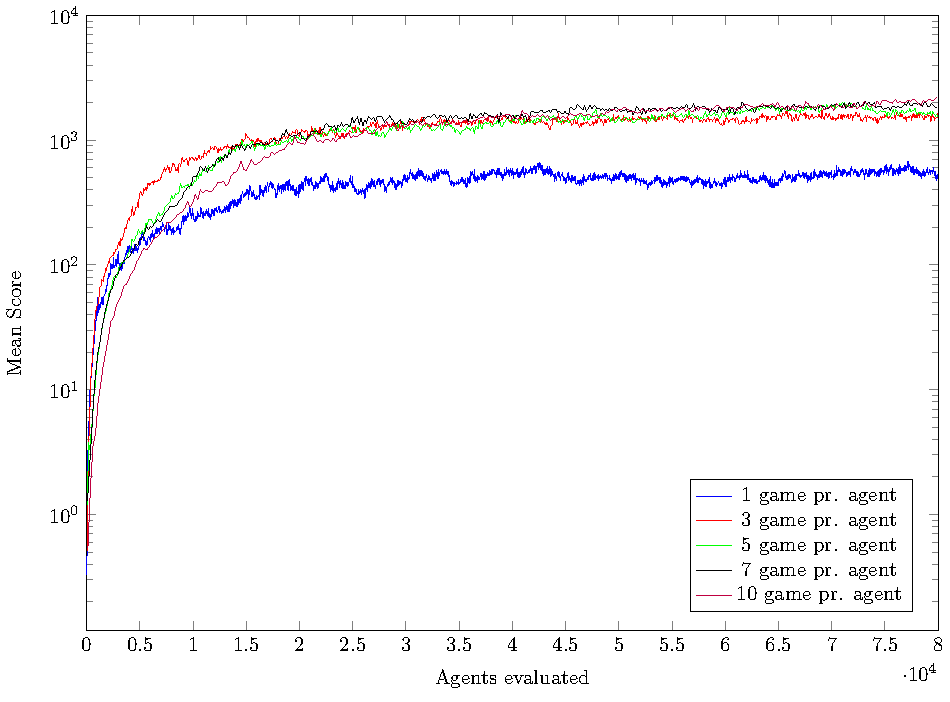
\includegraphics[width=\textwidth]{data/ce_population_offspring/12x_split/constant_l12_o6/mean/PlotFile.pdf}
    \end{subfigure}
    \begin{subfigure}[b]{0.49\textwidth}
    	\caption{Population size 22, Parent size 2}
        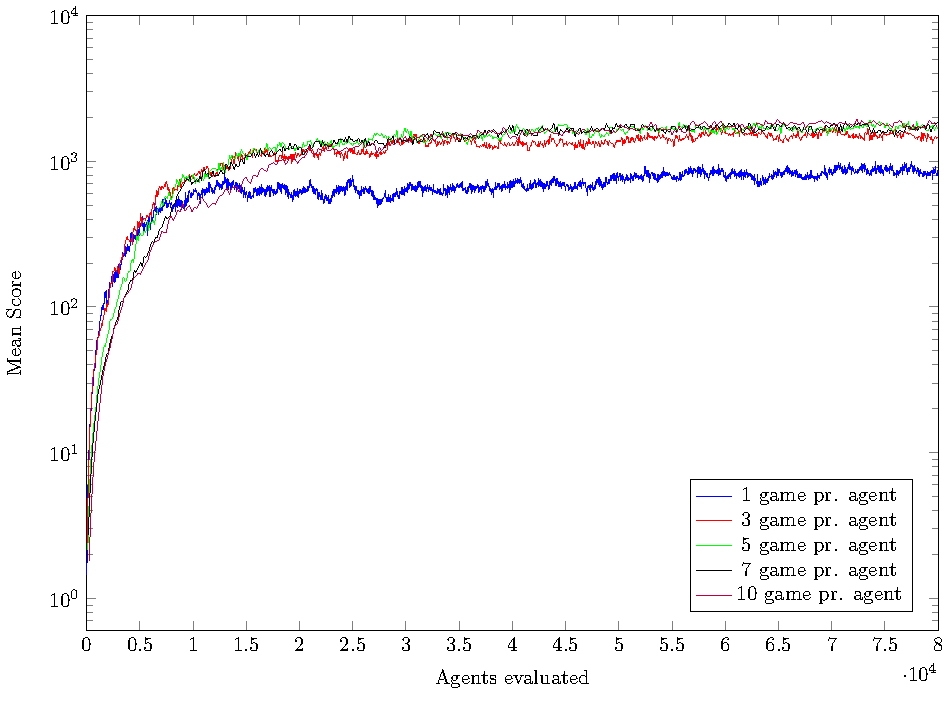
\includegraphics[width=\textwidth]{data/ce_population_offspring/22x_split/constant_l22_o2/mean/PlotFile.pdf}
    \end{subfigure}
    \begin{subfigure}[b]{0.49\textwidth}
    	\caption{Population size 22, Parent size 5}
        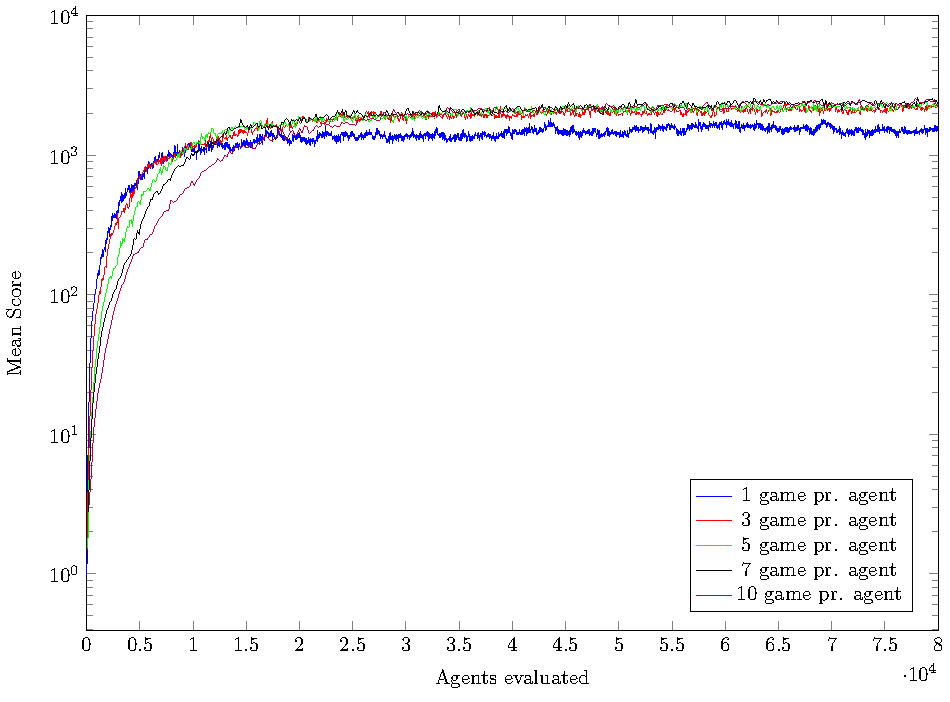
\includegraphics[width=\textwidth]{data/ce_population_offspring/22x_split/constant_l22_o5/mean/PlotFile.pdf}
    \end{subfigure}
    \begin{subfigure}[b]{0.49\textwidth}
    	\caption{Population size 22, Parent size 11}
        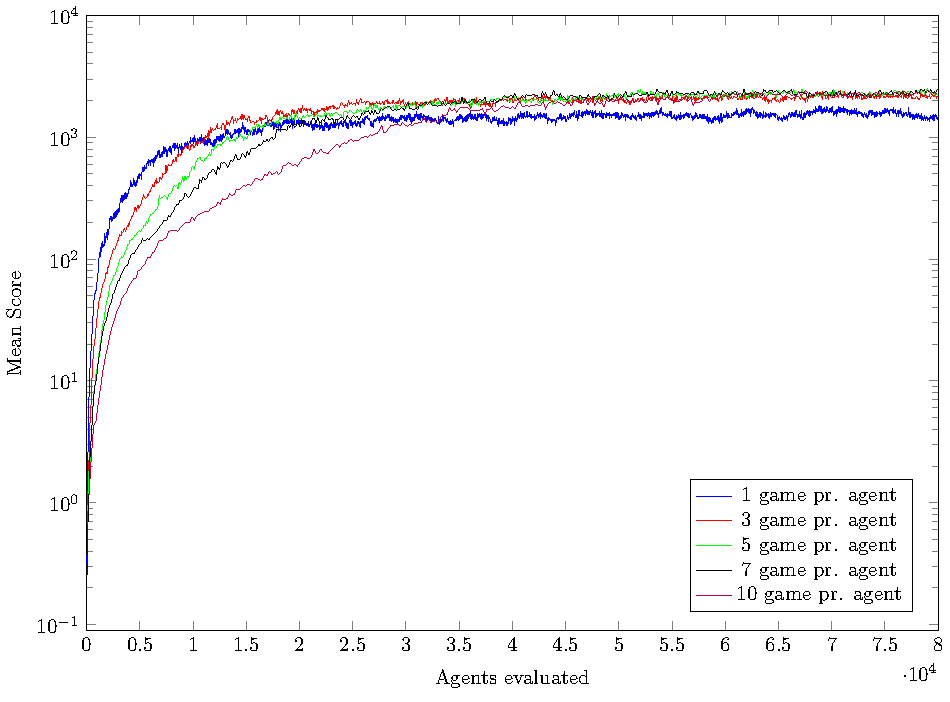
\includegraphics[width=\textwidth]{data/ce_population_offspring/22x_split/constant_l22_o11/mean/PlotFile.pdf}
    \end{subfigure}
    
    \caption{Mean results for population size 12 and 22 with parent sizes $10 \% , 25 \%$ and $50 \%$}
\end{figure}

\clearpage

\begin{figure}
	\centering
	\captionsetup[subfigure]{justification=centering}
    \begin{subfigure}[b]{0.49\textwidth}
    	\caption{Population size 50, Parent size 5}
        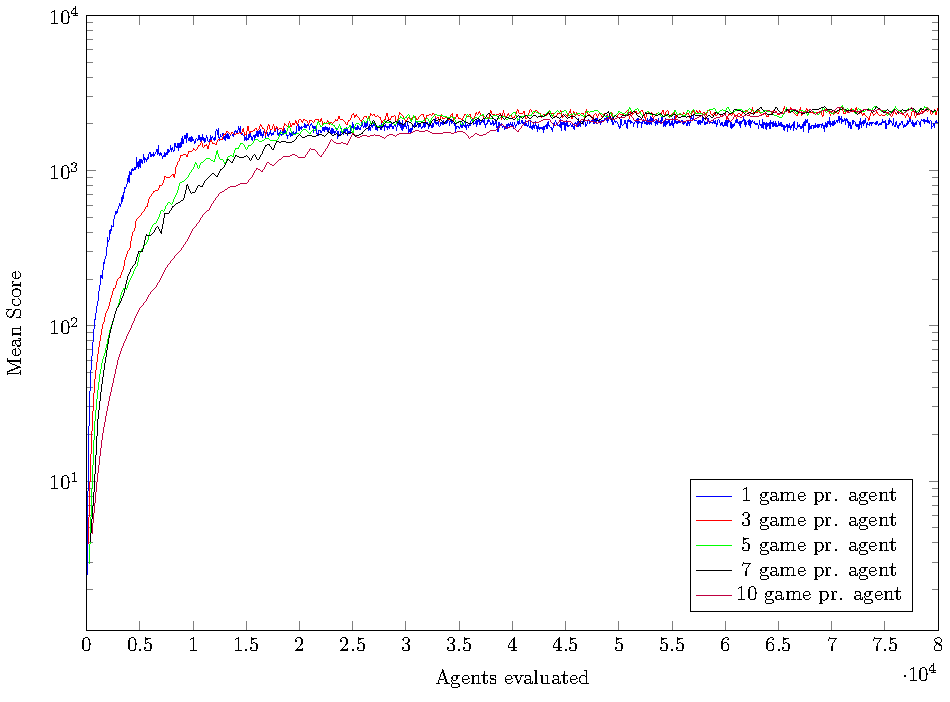
\includegraphics[width=\textwidth]{data/ce_population_offspring/50x_split/constant_l50_o5/mean/PlotFile.pdf}
    \end{subfigure} 
    \begin{subfigure}[b]{0.49\textwidth}
    	\caption{Population size 50, Parent size 12}
        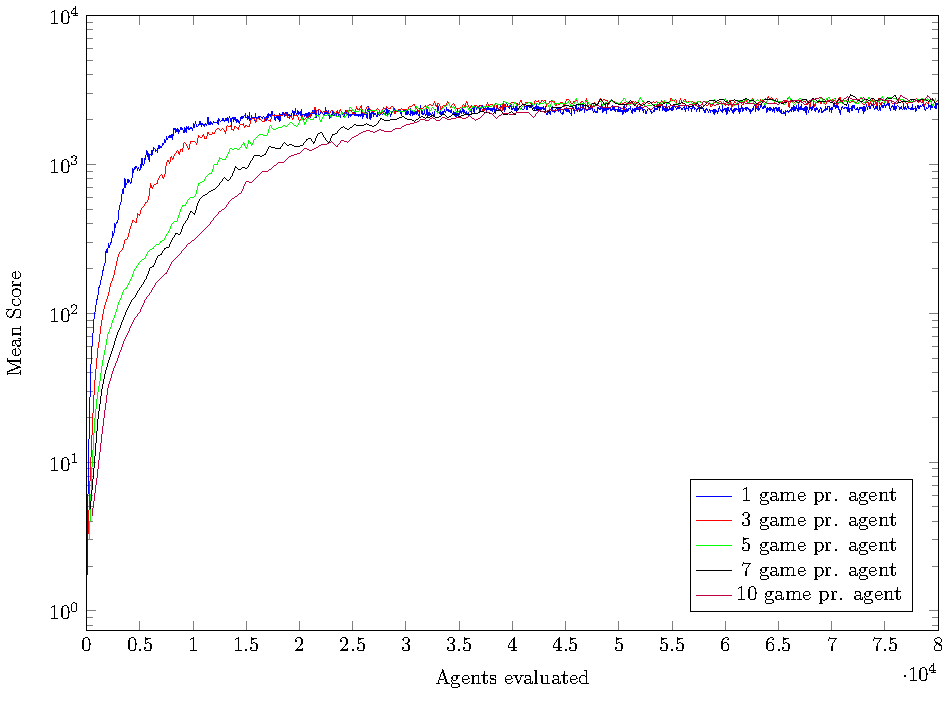
\includegraphics[width=\textwidth]{data/ce_population_offspring/50x_split/constant_l50_o12/mean/PlotFile.pdf}
    \end{subfigure}
    \begin{subfigure}[b]{0.49\textwidth}
    	\caption{Population size 50, Parent size 25}
        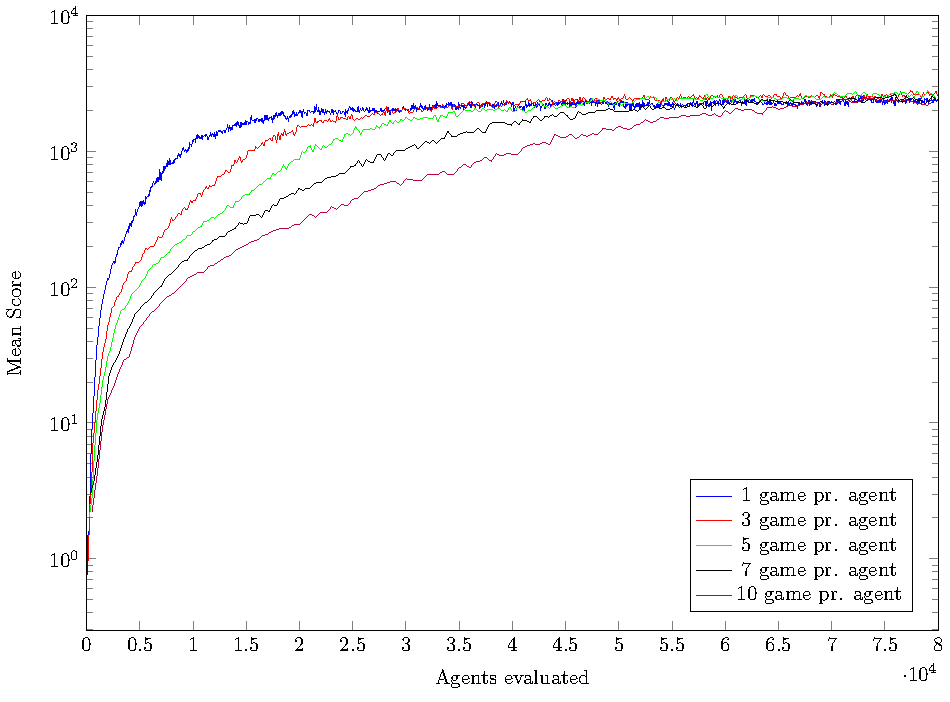
\includegraphics[width=\textwidth]{data/ce_population_offspring/50x_split/constant_l50_o25/mean/PlotFile.pdf}
    \end{subfigure}
    \begin{subfigure}[b]{0.49\textwidth}
    	\caption{Population size 100, Parent size 10}
        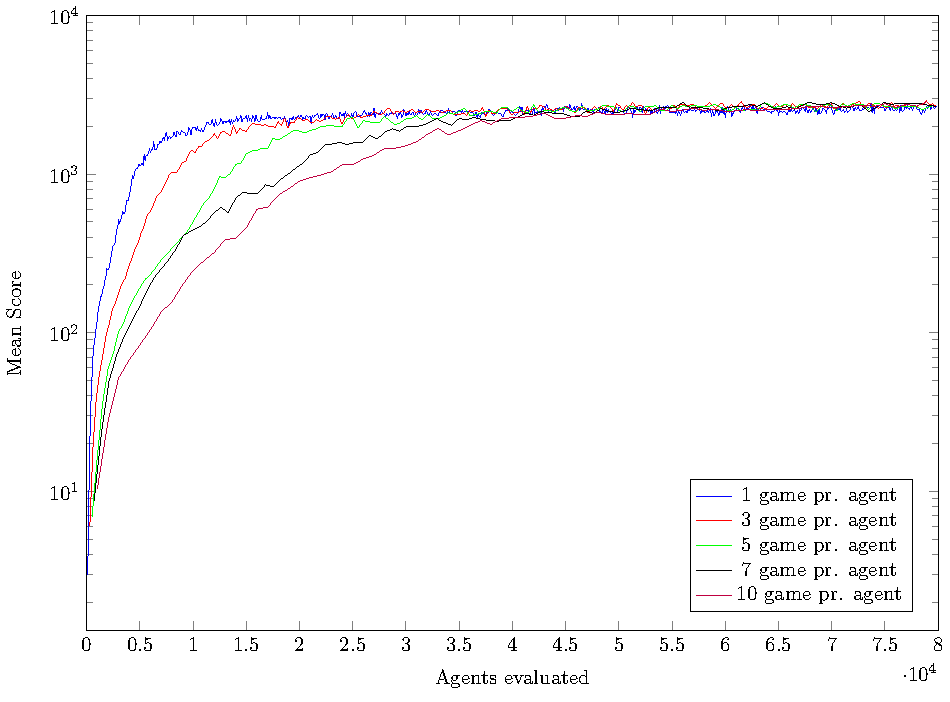
\includegraphics[width=\textwidth]{data/ce_population_offspring/100x_split/constant_l100_o10/mean/PlotFile.pdf}
    \end{subfigure}
    \begin{subfigure}[b]{0.49\textwidth}
    	\caption{Population size 100, Parent size 25}
        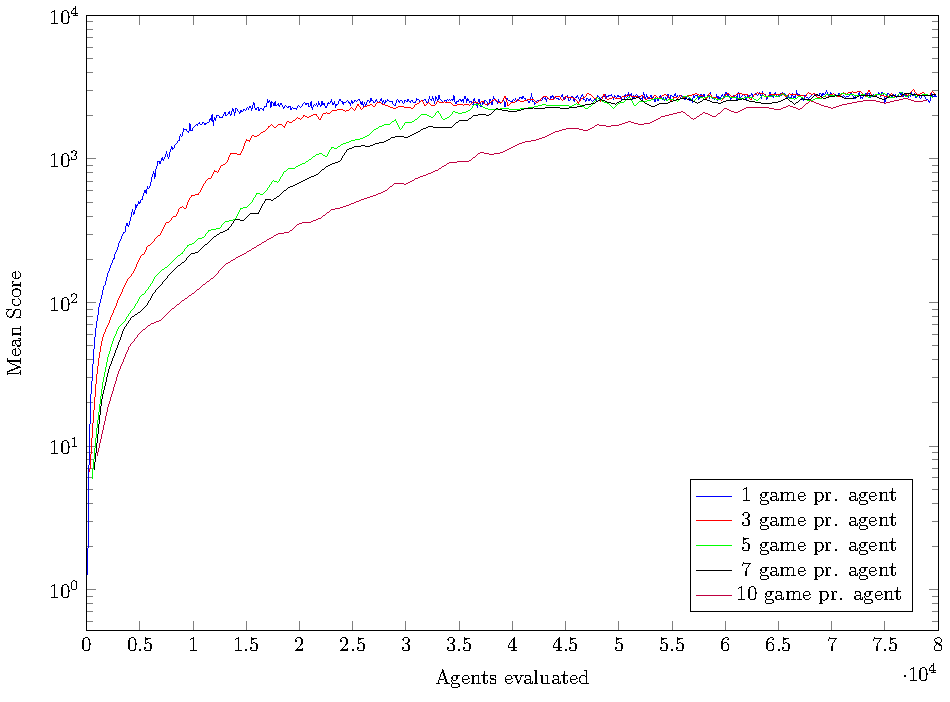
\includegraphics[width=\textwidth]{data/ce_population_offspring/100x_split/constant_l100_o25/mean/PlotFile.pdf}
    \end{subfigure}
    \begin{subfigure}[b]{0.49\textwidth}
    	\caption{Population size 100, Parent size 50}
        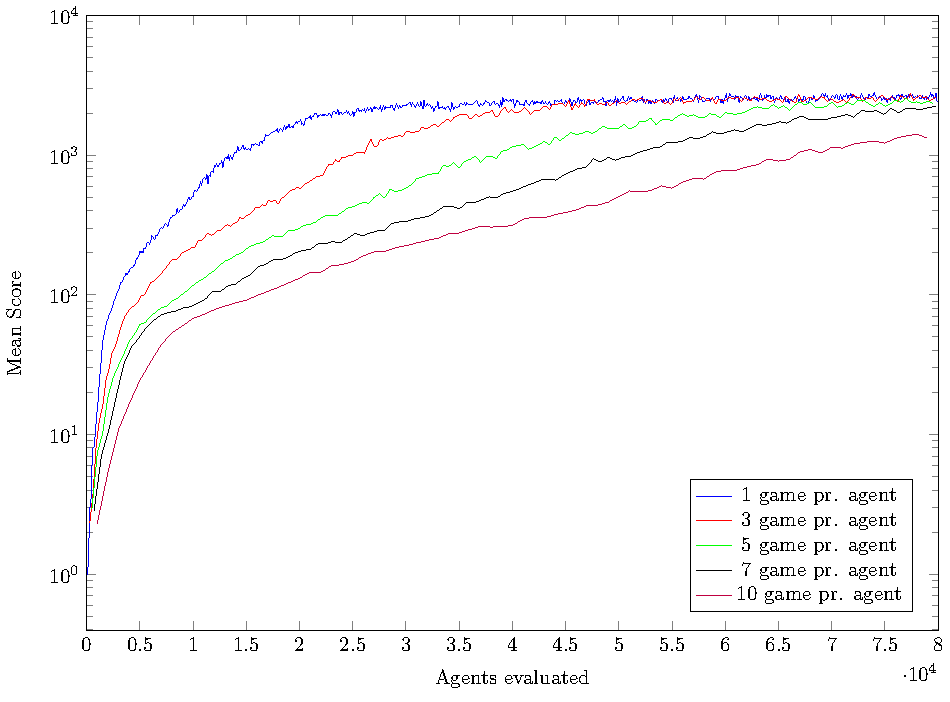
\includegraphics[width=\textwidth]{data/ce_population_offspring/100x_split/constant_l100_o50/mean/PlotFile.pdf}
    \end{subfigure}
    
    \caption{Mean results for population size 50 and 100 with parent sizes $10 \% , 25 \%$ and $50 \%$}
\end{figure}

\clearpage

\begin{figure}
	\captionsetup[subfigure]{justification=centering}
    \begin{subfigure}[b]{0.49\textwidth}
    	\caption{Population size 200, Parent size 20}
        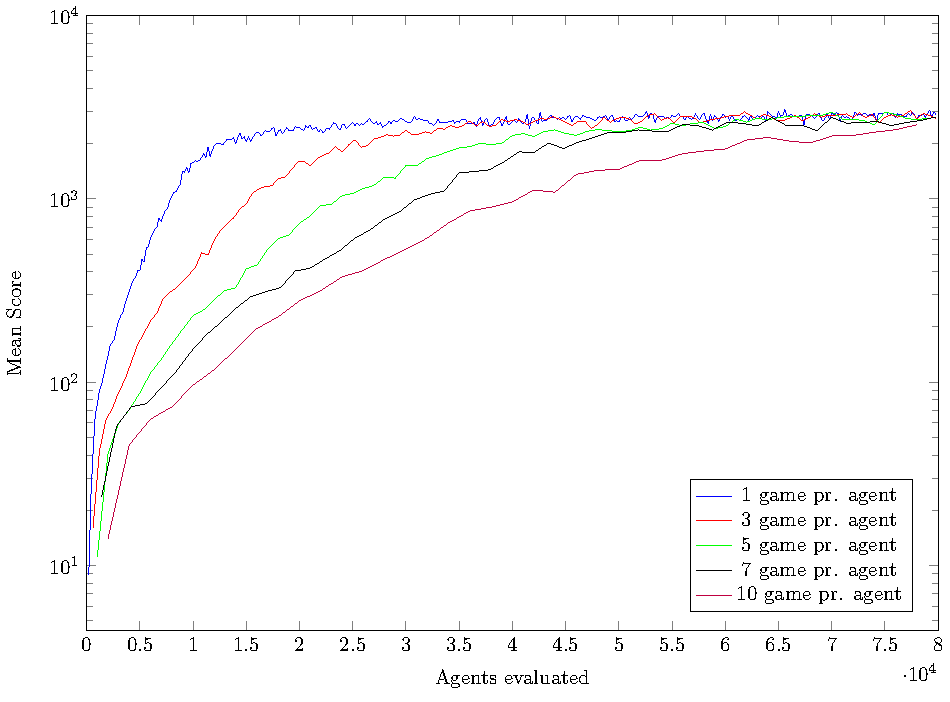
\includegraphics[width=\textwidth]{data/ce_population_offspring/200x_split/constant_l200_o20/mean/PlotFile.pdf}
    \end{subfigure} 
    \begin{subfigure}[b]{0.49\textwidth}
    	\caption{Population size 200, Parent size 50}
        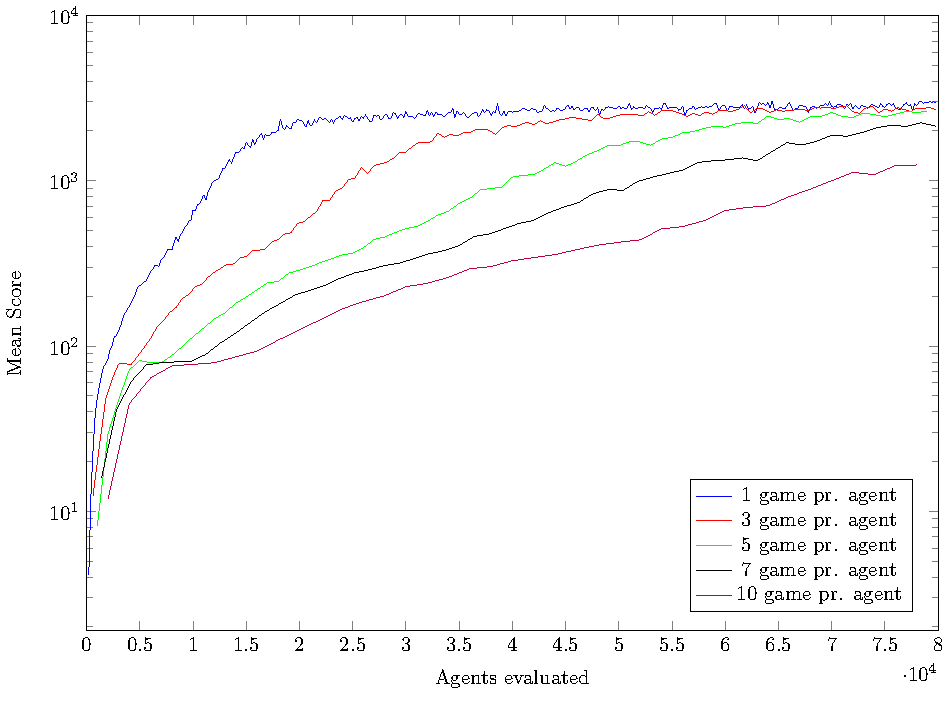
\includegraphics[width=\textwidth]{data/ce_population_offspring/200x_split/constant_l200_o50/mean/PlotFile.pdf}
    \end{subfigure}
    \begin{subfigure}[b]{0.49\textwidth}
    	\caption{Population size 200, Parent size 100}
        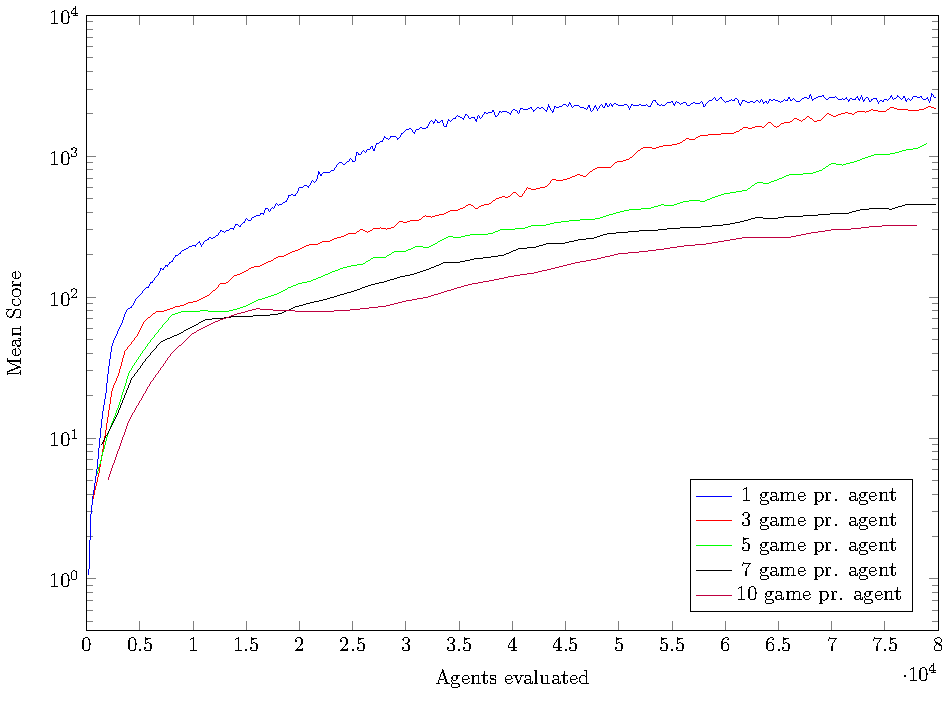
\includegraphics[width=\textwidth]{data/ce_population_offspring/200x_split/constant_l200_o100/mean/PlotFile.pdf}
    \end{subfigure}
    
    \caption{Mean results for population size 200 with parent sizes $10 \% , 25 \%$ and $50 \%$}
\end{figure}

\clearpage

\begin{table}[H]
\centering
\small
\begin{tabular}{c c c r r r r}
Population & Parent & Games per Agent & mean & Q1 & Q2 & Q3\\
\hline
$12$ & $1$ & 1 & $57.818$ & $46.277$ & $58.650$ & $72.703$\\
$12$ & $1$ & 3 & $356.373$ & $167.527$ & $271.933$ & $408.820$\\
$12$ & $1$ & 5 & $673.571$ & $411.463$ & $563.983$ & $834.717$\\
$12$ & $1$ & 7 & $942.772$ & $586.771$ & $819.434$ & $1249.562$\\
\hdashline
$12$ & $1$ & 10 & $1008.984$ & $724.373$ & $960.684$ & $1156.081$\\
\hdashline
$12$ & $3$ & 1 & - & - & - & -\\
$12$ & $3$ & 3 & - & - & - & -\\
$12$ & $3$ & 5 & - & - & - & -\\
\hdashline
$12$ & $3$ & 7 & - & - & - & -\\
\hdashline
$12$ & $3$ & 10 & - & - & - & -\\
$12$ & $6$ & 1 & $510.686$ & $305.133$ & $421.067$ & $630.730$\\
$12$ & $6$ & 3 & $1584.396$ & $1359.411$ & $1479.835$ & $1651.791$\\
$12$ & $6$ & 5 & $1524.285$ & $1349.078$ & $1597.585$ & $1728.091$\\
$12$ & $6$ & 7 & $1824.980$ & $1568.218$ & $1767.685$ & $2035.880$\\
\hdashline
$12$ & $6$ & 10 & $2109.837$ & $1802.968$ & $2021.165$ & $2276.652$\\
\hdashline
\end{tabular}
\caption{population 12 - Cross Entropy}
\end{table}

\begin{table}[H]
\centering
\small
\begin{tabular}{c c c r r r r}
Population & Parent & Games per Agent & mean & Q1 & Q2 & Q3\\
\hline
$22$ & $2$ & 1 & $849.001$ & $542.797$ & $799.083$ & $1031.299$\\
$22$ & $2$ & 3 & $1442.883$ & $1276.870$ & $1437.550$ & $1541.938$\\
$22$ & $2$ & 5 & $1668.974$ & $1352.250$ & $1579.885$ & $1849.210$\\
\hdashline
$22$ & $2$ & 7 & $1843.644$ & $1575.732$ & $1860.815$ & $2112.678$\\
\hdashline
$22$ & $2$ & 10 & $1732.664$ & $1475.000$ & $1754.785$ & $2024.980$\\
$22$ & $5$ & 1 & $1485.692$ & $1202.661$ & $1561.635$ & $1661.268$\\
$22$ & $5$ & 3 & $2250.239$ & $2081.798$ & $2210.850$ & $2435.021$\\
\hdashline
$22$ & $5$ & 5 & $2371.793$ & $2013.168$ & $2412.815$ & $2708.931$\\
\hdashline
$22$ & $5$ & 7 & $2351.371$ & $1976.141$ & $2274.180$ & $2586.641$\\
$22$ & $5$ & 10 & $2266.329$ & $2010.798$ & $2175.850$ & $2365.220$\\
$22$ & $11$ & 1 & $1415.511$ & $1011.101$ & $1327.030$ & $1600.599$\\
$22$ & $11$ & 3 & $2168.012$ & $1966.552$ & $2119.100$ & $2456.230$\\
$22$ & $11$ & 5 & $2245.854$ & $2017.992$ & $2222.900$ & $2424.450$\\
\hdashline
$22$ & $11$ & 7 & $2463.227$ & $2091.090$ & $2384.230$ & $2702.740$\\
\hdashline
$22$ & $11$ & 10 & $2282.032$ & $1957.148$ & $2257.285$ & $2565.950$\\
\end{tabular}
\caption{population 22 - Cross Entropy}
\end{table}


\begin{table}[H]
\centering
\small
\begin{tabular}{c c c r r r r}
Population & Parent & Games per Agent & mean & Q1 & Q2 & Q3\\
\hline
$50$ & $5$ & 1 & $2060.069$ & $1731.441$ & $1967.465$ & $2076.389$\\
\hdashline
$50$ & $5$ & 3 & $2524.279$ & $2195.189$ & $2501.985$ & $2848.859$\\
\hdashline
$50$ & $5$ & 5 & $2418.023$ & $2283.708$ & $2388.770$ & $2639.078$\\
$50$ & $5$ & 7 & $2433.615$ & $2145.718$ & $2356.800$ & $2734.611$\\
$50$ & $5$ & 10 & $2341.267$ & $2104.480$ & $2252.570$ & $2418.809$\\
$50$ & $12$ & 1 & $2563.539$ & $2283.399$ & $2502.880$ & $2830.192$\\
$50$ & $12$ & 3 & $2702.266$ & $2322.849$ & $2565.365$ & $2841.160$\\
\hdashline
$50$ & $12$ & 5 & $2749.991$ & $2605.171$ & $2702.400$ & $2835.960$\\
\hdashline
$50$ & $12$ & 7 & $2527.792$ & $2287.091$ & $2476.965$ & $2758.970$\\
$50$ & $12$ & 10 & $2687.438$ & $2342.811$ & $2577.285$ & $2838.771$\\
$50$ & $25$ & 1 & $2396.866$ & $2115.161$ & $2357.980$ & $2664.099$\\
\hdashline
$50$ & $25$ & 3 & $2572.860$ & $2308.748$ & $2615.185$ & $2861.858$\\
\hdashline
$50$ & $25$ & 5 & $2485.564$ & $2226.889$ & $2419.080$ & $2747.609$\\
$50$ & $25$ & 7 & $2396.309$ & $2180.099$ & $2306.165$ & $2605.832$\\
$50$ & $25$ & 10 & $2332.305$ & $2019.738$ & $2268.415$ & $2561.252$\\
\end{tabular}
\caption{population 50 - Cross Entropy}
\end{table}



\begin{table}[H]
\centering
\small
\begin{tabular}{c c c r r r r}
Population & Parent & Games per Agent & mean & Q1 & Q2 & Q3\\
\hline
$100$ & $10$ & 1 & $2658.689$ & $2469.169$ & $2601.480$ & $2866.970$\\
$100$ & $10$ & 3 & $2677.629$ & $2375.419$ & $2770.615$ & $3004.819$\\
$100$ & $10$ & 5 & $2690.802$ & $2360.800$ & $2646.920$ & $2946.831$\\
$100$ & $10$ & 7 & $2678.393$ & $2442.688$ & $2630.120$ & $2877.830$\\
\hdashline
$100$ & $10$ & 10 & $2880.385$ & $2636.640$ & $2828.880$ & $3108.429$\\
\hdashline
$100$ & $25$ & 1 & $2702.678$ & $2443.269$ & $2692.620$ & $2973.202$\\
\hdashline
$100$ & $25$ & 3 & $2776.560$ & $2397.691$ & $2742.950$ & $3027.541$\\
\hdashline
$100$ & $25$ & 5 & $2666.479$ & $2469.161$ & $2673.770$ & $2917.939$\\
$100$ & $25$ & 7 & $2555.354$ & $2187.871$ & $2461.220$ & $2866.030$\\
$100$ & $25$ & 10 & $2823.755$ & $2540.171$ & $2729.280$ & $2933.510$\\
$100$ & $50$ & 1 & $2409.168$ & $2206.828$ & $2299.435$ & $2534.019$\\
\hdashline
$100$ & $50$ & 3 & $2622.402$ & $2318.410$ & $2714.500$ & $2905.521$\\
\hdashline
$100$ & $50$ & 5 & $2351.742$ & $2213.480$ & $2410.500$ & $2532.500$\\
$100$ & $50$ & 7 & $2232.970$ & $2035.291$ & $2296.430$ & $2466.811$\\
$100$ & $50$ & 10 & $1320.906$ & $1088.809$ & $1231.050$ & $1618.431$\\
\end{tabular}
\caption{population 100 - Cross Entropy}
\end{table}


\begin{table}[H]
\centering
\small
\begin{tabular}{c c c r r r r}
Population & Parent & Games per Agent & mean & Q1 & Q2 & Q3\\
\hline
\hdashline
$200$ & $20$ & 1 & $2880.572$ & $2596.999$ & $2764.400$ & $3184.290$\\
\hdashline
$200$ & $20$ & 3 & $2735.539$ & $2493.400$ & $2751.215$ & $2849.329$\\
$200$ & $20$ & 5 & $2756.202$ & $2609.579$ & $2728.885$ & $2826.881$\\
$200$ & $20$ & 7 & $2797.015$ & $2515.971$ & $2722.150$ & $3036.839$\\
$200$ & $20$ & 10 & $2531.674$ & $2186.629$ & $2652.365$ & $2897.672$\\
\hdashline
$200$ & $50$ & 1 & $2950.767$ & $2564.118$ & $2841.065$ & $3377.189$\\
\hdashline
$200$ & $50$ & 3 & $2677.694$ & $2414.600$ & $2559.765$ & $2803.289$\\
$200$ & $50$ & 5 & $2627.598$ & $2296.710$ & $2641.415$ & $2999.199$\\
$200$ & $50$ & 7 & $2140.359$ & $1884.261$ & $2173.235$ & $2418.772$\\
$200$ & $50$ & 10 & $1245.519$ & $625.930$ & $1009.132$ & $1644.630$\\
\hdashline
$200$ & $100$ & 1 & $2589.020$ & $2391.080$ & $2594.285$ & $2798.470$\\
\hdashline
$200$ & $100$ & 3 & $2164.732$ & $2018.790$ & $2136.900$ & $2335.079$\\
$200$ & $100$ & 5 & $1235.709$ & $837.947$ & $1195.730$ & $1478.081$\\
$200$ & $100$ & 7 & $451.171$ & $377.813$ & $421.150$ & $498.470$\\
$200$ & $100$ & 10 & $320.356$ & $287.023$ & $322.733$ & $350.773$\\
\end{tabular}
\caption{population 200 - Cross Entropy}
\end{table}

\clearpage

\begin{table}[H]
\centering
\small
\begin{tabular}{c c c r r r r}
Population & Parent & Games per Agent & mean & Q1 & Q2 & Q3\\
\hline
$12$ & $1$ & 10 & $1008.984$ & $724.373$ & $960.684$ & $1156.081$\\
$12$ & $3$ & 7 & - & - & - & -\\
$12$ & $6$ & 10 & $2109.837$ & $1802.968$ & $2021.165$ & $2276.652$\\
\end{tabular}
\caption{population 12 - Cross Entropy}
\end{table}

\begin{figure}[H]
\centering
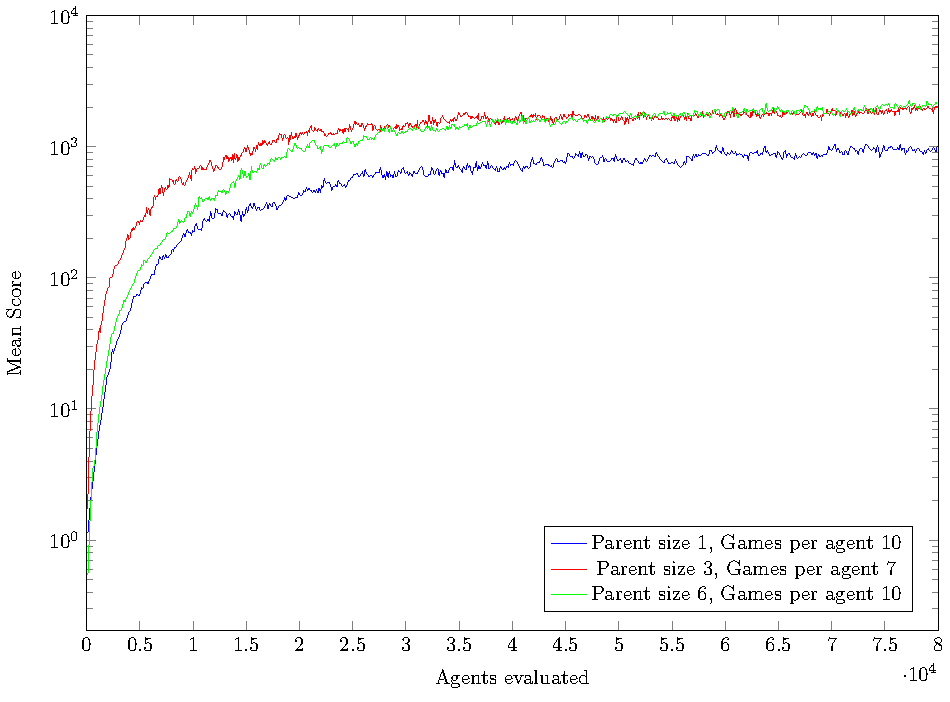
\includegraphics[scale=1]{data/ce_population_offspring/bestofeach_population/12x/PlotFile.pdf}
\caption{Best performing configurations for population size 12}
\end{figure}

\clearpage

\begin{table}[H]
\centering
\small
\begin{tabular}{c c c r r r r}
Population & Parent & Games per Agent & mean & Q1 & Q2 & Q3\\
\hline
$22$ & $2$ & 7 & $1843.644$ & $1575.732$ & $1860.815$ & $2112.678$\\
$22$ & $5$ & 5 & $2371.793$ & $2013.168$ & $2412.815$ & $2708.931$\\
$22$ & $11$ & 7 & $2463.227$ & $2091.090$ & $2384.230$ & $2702.740$\\
\end{tabular}
\caption{population 22 - Cross Entropy}
\end{table}

\begin{figure}[H]
\centering
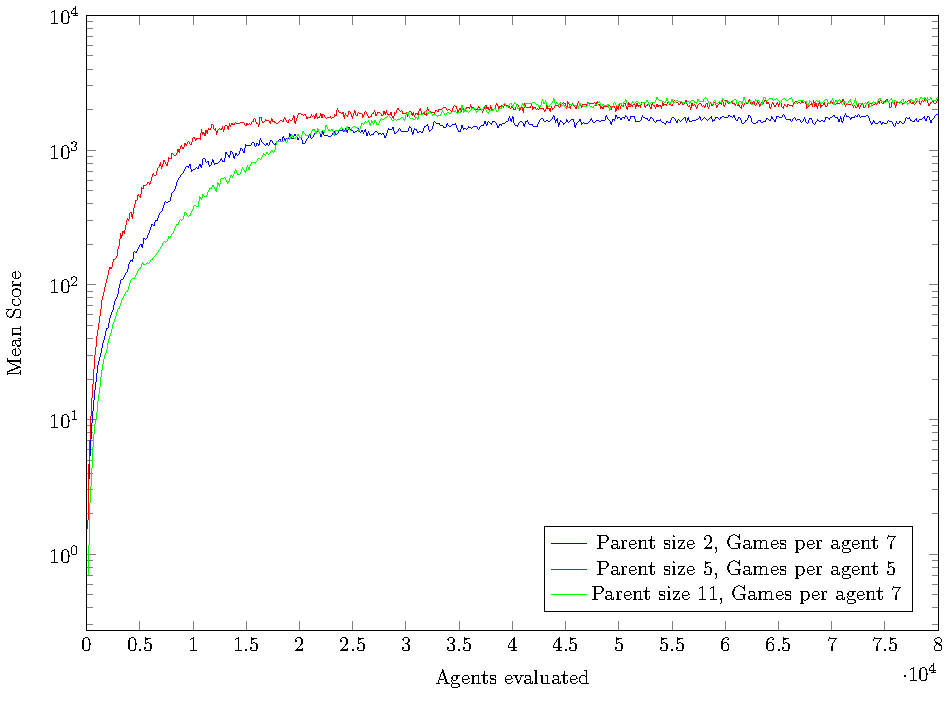
\includegraphics[scale=1]{data/ce_population_offspring/bestofeach_population/22x/PlotFile.pdf}
\caption{Best performing configurations for population size 22}
\end{figure}

\clearpage

\begin{table}[H]
\centering
\small
\begin{tabular}{c c c r r r r}
Population & Parent & Games per Agent & mean & Q1 & Q2 & Q3\\
\hline
$50$ & $5$ & 3 & $2524.279$ & $2195.189$ & $2501.985$ & $2848.859$\\
$50$ & $12$ & 5 & $2749.991$ & $2605.171$ & $2702.400$ & $2835.960$\\
$50$ & $25$ & 3 & $2572.860$ & $2308.748$ & $2615.185$ & $2861.858$\\
\end{tabular}
\caption{population 50 - Cross Entropy}
\end{table}

\begin{figure}[H]
\centering
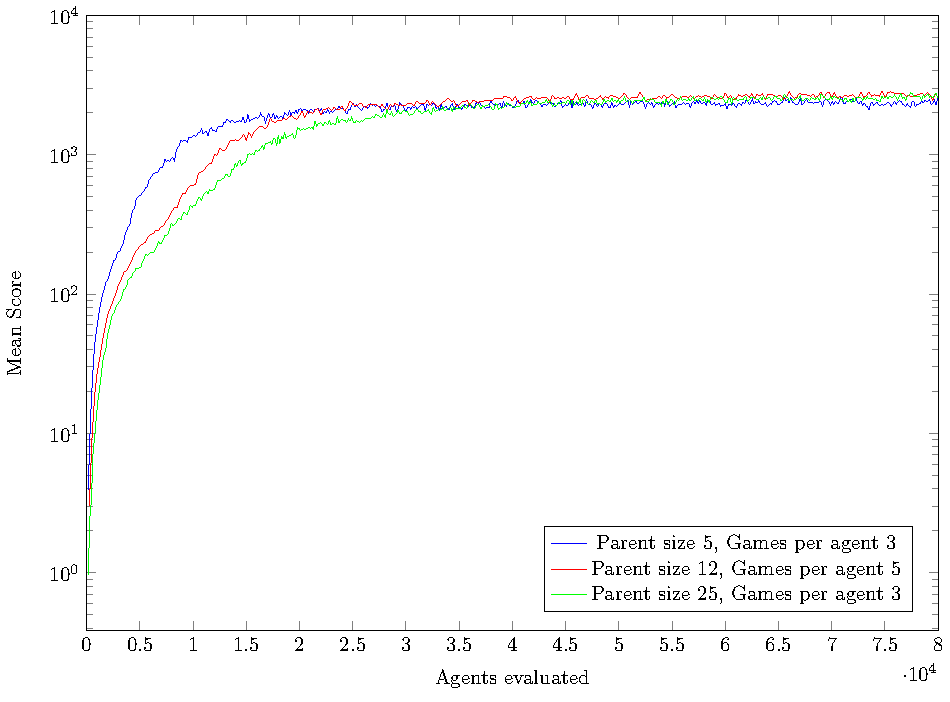
\includegraphics[scale=1]{data/ce_population_offspring/bestofeach_population/50x/PlotFile.pdf}
\caption{Best performing configurations for population size 50}
\end{figure}

\clearpage

\begin{table}[H]
\centering
\small
\begin{tabular}{c c c r r r r}
Population & Parent & Games per Agent & mean & Q1 & Q2 & Q3\\
\hline
$100$ & $10$ & 10 & $2880.385$ & $2636.640$ & $2828.880$ & $3108.429$\\
$100$ & $25$ & 3 & $2776.560$ & $2397.691$ & $2742.950$ & $3027.541$\\
$100$ & $50$ & 3 & $2622.402$ & $2318.410$ & $2714.500$ & $2905.521$\\
\end{tabular}
\caption{population 100 - Cross Entropy}
\end{table}

\begin{figure}[H]
\centering
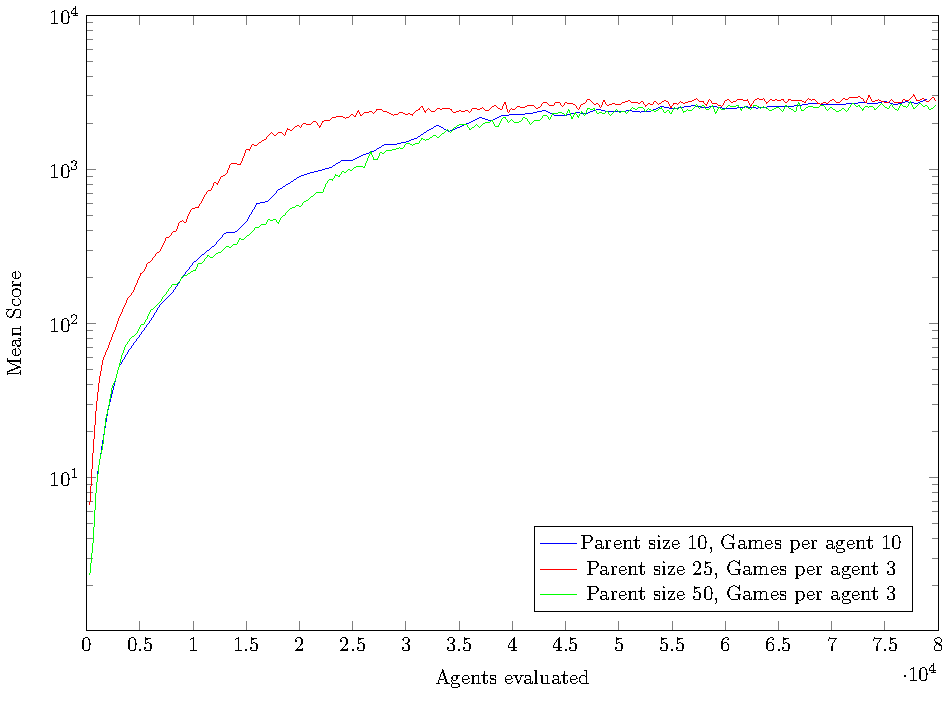
\includegraphics[scale=1]{data/ce_population_offspring/bestofeach_population/100x/PlotFile.pdf}
\caption{Best performing configurations for population size 100}
\end{figure}

\clearpage

\begin{table}[H]
\centering
\small
\begin{tabular}{c c c r r r r}
Population & Parent & Games per Agent & mean & Q1 & Q2 & Q3\\
\hline
$200$ & $20$ & 1 & $2880.572$ & $2596.999$ & $2764.400$ & $3184.290$\\
$200$ & $50$ & 1 & $2950.767$ & $2564.118$ & $2841.065$ & $3377.189$\\
$200$ & $100$ & 1 & $2589.020$ & $2391.080$ & $2594.285$ & $2798.470$\\
\end{tabular}
\caption{population 200 - Cross Entropy}
\end{table}

\begin{figure}[H]
\centering
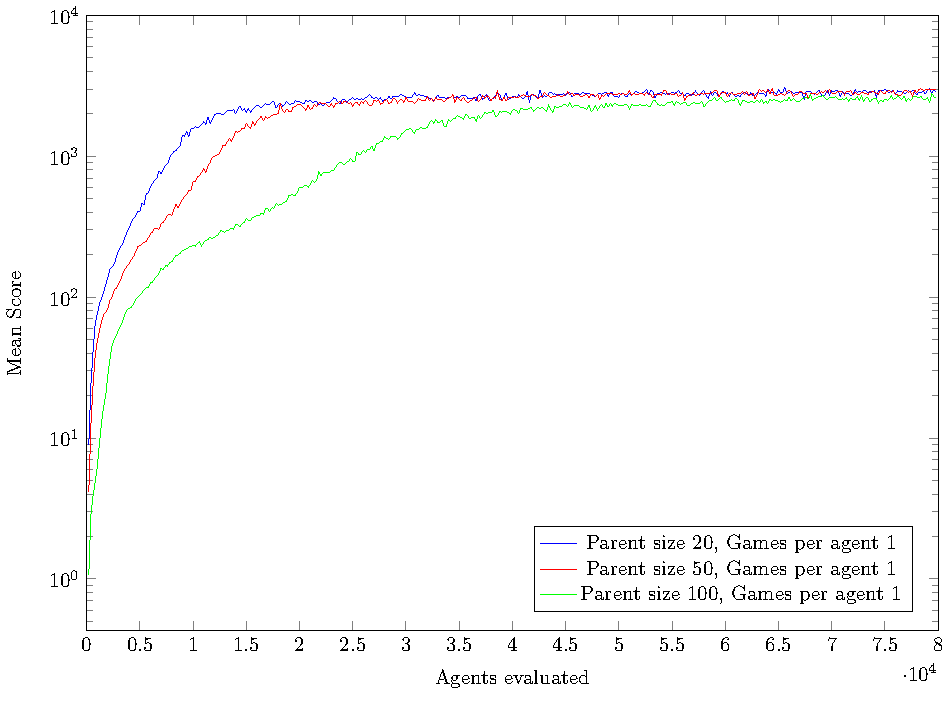
\includegraphics[scale=1]{data/ce_population_offspring/bestofeach_population/200x/PlotFile.pdf}
\caption{Best performing configurations for population size 200}
\end{figure}

\clearpage

\begin{table}[H]
\centering
\small
\begin{tabular}{c c c r r r r}
Population & Parent & Games per Agent & mean & Q1 & Q2 & Q3\\
\hline
$12$ & $6$ & 10 & $2109.837$ & $1802.968$ & $2021.165$ & $2276.652$\\
$22$ & $5$ & 5 & $2371.793$ & $2013.168$ & $2412.815$ & $2708.931$\\
$50$ & $12$ & 5 & $2749.991$ & $2605.171$ & $2702.400$ & $2835.960$\\
$100$ & $25$ & 3 & $2776.560$ & $2397.691$ & $2742.950$ & $3027.541$\\
$200$ & $50$ & 1 & $2950.767$ & $2564.118$ & $2841.065$ & $3377.189$\\
\end{tabular}
\caption{Best configurations of all population sizes - Cross Entropy}
\end{table}

\begin{figure}[H]
\centering
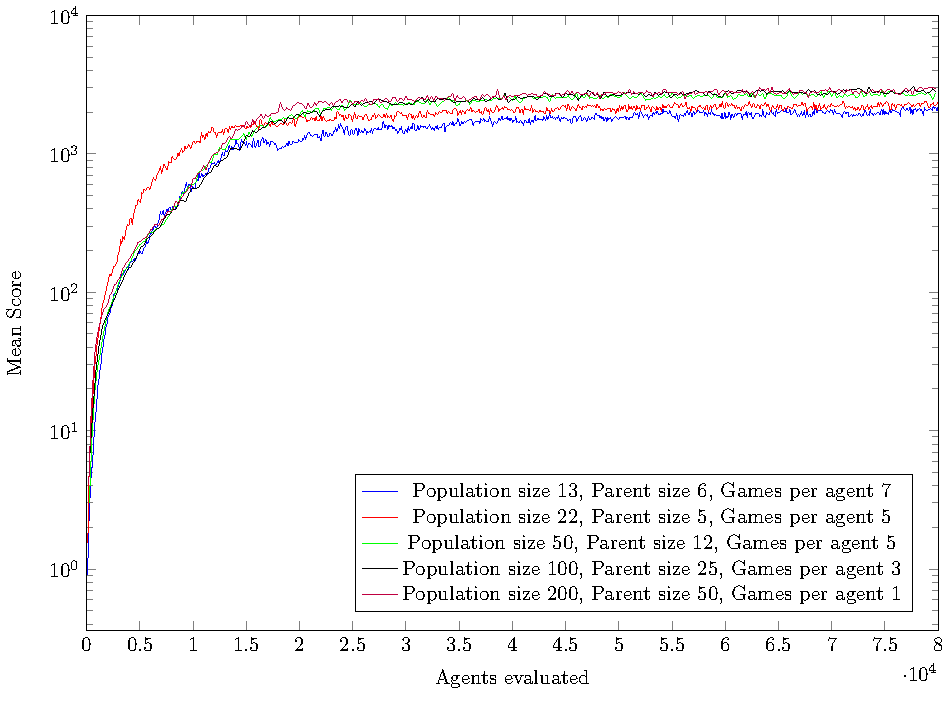
\includegraphics[scale=1]{data/ce_population_offspring/bestofall_population/PlotFile.pdf}
\caption{Best configurations of all population sizes - Cross Entropy}
\end{figure}


\clearpage

\subsection{Optimal settings for CMA - Initial Step-size}
Experiments to find the best initial step-size for CMA.

\begin{table}[h]
\centering
\caption{Overview of the two table formats}
\begin{tabular}{l r}
Optimizer & CMA\\
Number of Evaluations & 8000\\
Number of Learning Games &30\\
Population size& 13\\
Parent size & 6\\
Games per Agent & 1\\
Tetris Type & Normal\\
\hline
Recombination Type & Superlinear\\
Initial Sigma & See table \ref{InitialSigmaTest}
\end{tabular}
\end{table}

with the following initial sigma

\begin{table}[H]
\centering
\begin{tabular}{c | c c c c c c}
$\sigma_0$ & 0.1 & 0.2 & 0.5 & 0.8 & 1.0
\end{tabular}
\caption{Initial sigma configurations \label{InitialSigmaTest}}
\end{table}

INSERT PLOTS HERE.\\
\\


\begin{figure}[H]
\centering
\begin{tabular}{r | r r r r r}
$\sigma_0$ & mean & Q1 & Q2 & Q3\\
\hline
0.1 & 50769.3 & 21301.1 & 54588.7 & 73972.4\\
0.2 & 42290.6 & 32180.2 & 42290.6 & 49337.4\\
0.5 & 53893.7 & 14211.1 & 66773.0 & 85816.7\\
0.8 & 37557.7 & 1422.8  & 15450.8 & 93719.4\\
1.0 & 49537.9 & 31369.8 & 49537.4 & 58454.6
\end{tabular}
\caption{Results of CMA-ES with adjusted initial step-size \label{CMAInitialSigmaConfigTestAppendix}}
\end{figure}

\clearpage

\subsection{Optimal settings for CMA - Experiment for finding the optimal settings \label{appendixCMAPopulationParent}}
Experiments finding the best configuration of population and parent size with recombination type. The parent size is dependent on the recombination type, therefore we tested these parameter together.
\begin{table}[h]
\centering
\begin{tabular}{l r}
Optimizer & CMA\\
Number of Evaluations & 80000\\
Number of Learning Games &30\\
Population size& See table \ref{SuperCMAExperiment}\\
Parent size & See table \ref{SuperCMAExperiment}\\
Games per Agent & See table \ref{SuperCMAExperiment}\\
Tetris Type & Hard\\
\hline
Recombination Type & See table \ref{SuperCMAExperiment}\\
Initial Sigma & 1
\end{tabular}
\caption{CMA experiment parameters for testing games per agent}
\end{table}

\begin{table}[H]
\centering
\begin{tabular}{c c l c}
Population Size & Parent size & Recombination Type & Games per Agent\\
\hline
$12$ & $1$ & EQUAL/LINEAR/SUPERLINEAR & 1/3/5/7/10\\
$12$ & $3$ & EQUAL & 1/3/5/7/10\\
$12$ & $6$ & LINEAR/SUPERLINEAR & 1/3/5/7/10\\
$22$ & $2$ & EQUAL/LINEAR/SUPERLINEAR & 1/3/5/7/10\\
$22$ & $5$ & EQUAL & 1/3/5/7/10\\
$22$ & $11$ & LINEAR/SUPERLINEAR & 1/3/5/7/10\\
$50$ & $5$ & EQUAL/LINEAR/SUPERLINEAR & 1/3/5/7/10\\
$50$ & $12$ & EQUAL & 1/3/5/7/10\\
$50$ & $25$ & LINEAR/SUPERLINEAR & 1/3/5/7/10\\
$100$ & $10$ & EQUAL/LINEAR/SUPERLINEAR & 1/3/5/7/10\\
$100$ & $25$ & EQUAL & 1/3/5/7/10\\
$100$ & $50$ & LINEAR/SUPERLINEAR & 1/3/5/7/10
\end{tabular}
\caption{Full experiments overview \label{SuperCMAExperimentAppendix}}
\end{table}


%\begin{figure}
%\centering
%\caption{Population size 12, Parent size 1, \\Meanscore of EQUAL recombination}
%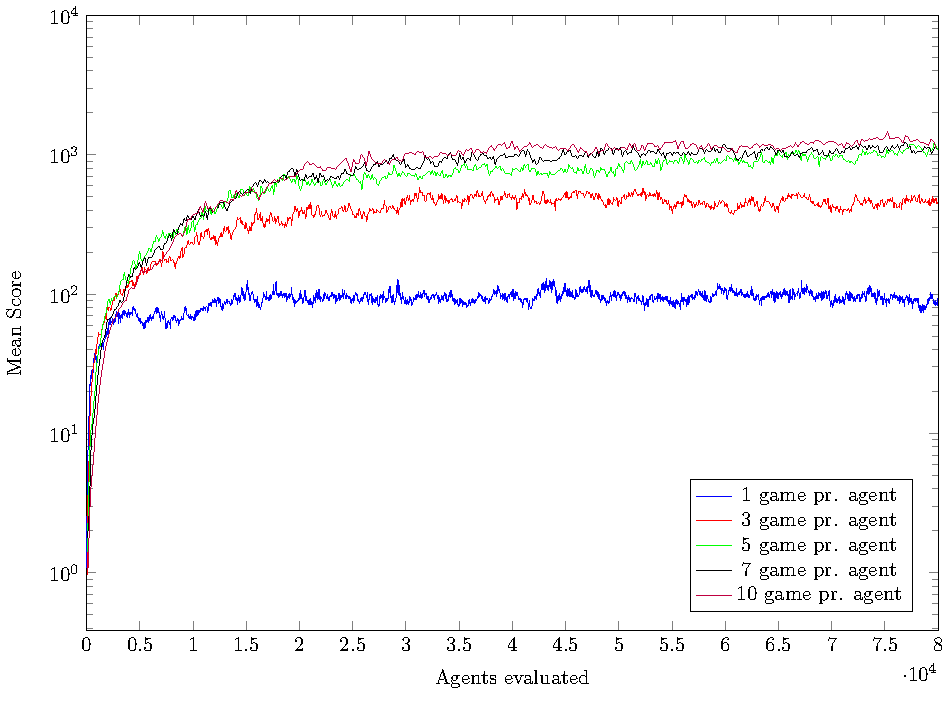
\includegraphics[scale=0.5]{data/cma_population_offspring/12x_split/equal_l12_o1/mean/PlotFile.pdf}
%\end{figure}

\comment{When only testing 1 game pr agent, we observe that after 8000 agents it starts to decline in
 score, thus finding worse performing agents - some conclusion that cma with 1 game pr agent should be
  run only for some time and not infinityly}
\comment{as seen on ex. population 12, parent size 6, linear, if played with dynamic games, meaning 1 game up to 500 agent and then a higher games per agent afterwards, a fast convergence and high score is achieved.}

\clearpage

\begin{figure}
	\centering
	\captionsetup[subfigure]{justification=centering}
    \begin{subfigure}[b]{0.49\textwidth}
    	\caption{Population size 12, Parent size 1,\\EQUAL recombination}
        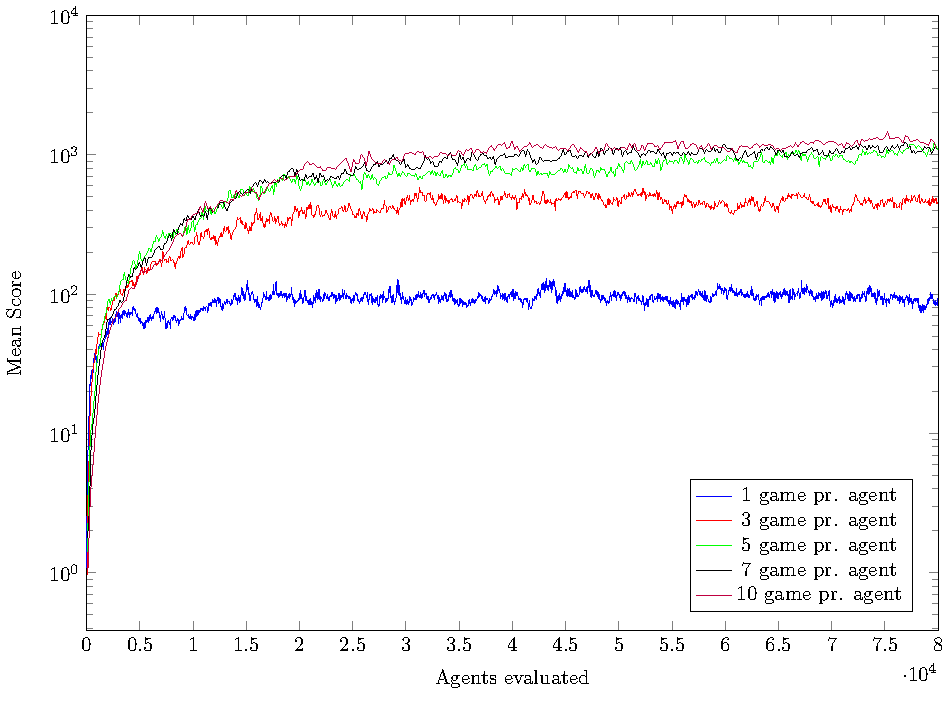
\includegraphics[width=\textwidth]{data/cma_population_offspring/12x_split/equal_l12_o1/mean/PlotFile.pdf}
    \end{subfigure} 
    \begin{subfigure}[b]{0.49\textwidth}
    	\caption{Population size 12, Parent size 3,\\EQUAL recombination}
        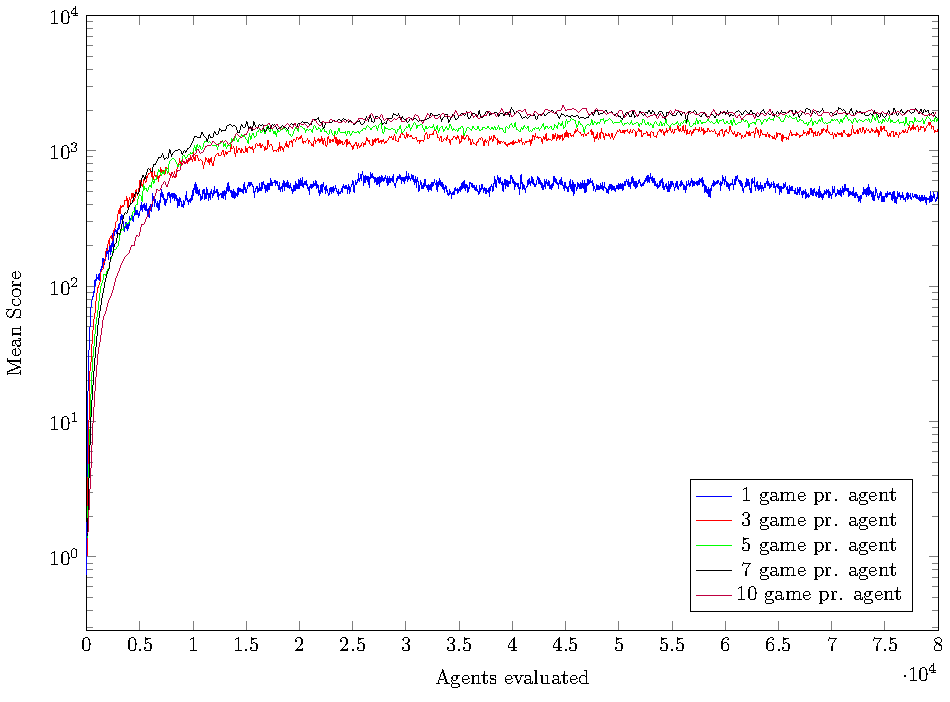
\includegraphics[width=\textwidth]{data/cma_population_offspring/12x_split/equal_l12_o3/mean/PlotFile.pdf}
    \end{subfigure}
    \begin{subfigure}[b]{0.49\textwidth}
    	\caption{Population size 12, Parent size 1,\\LINEAR recombination}
        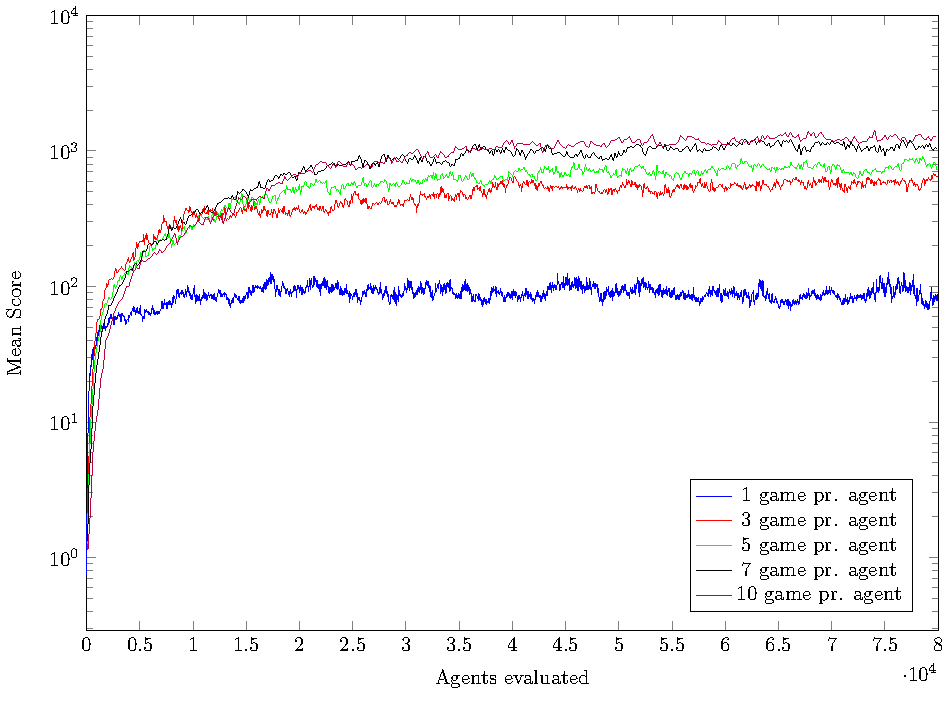
\includegraphics[width=\textwidth]{data/cma_population_offspring/12x_split/linear_l12_o1/mean/PlotFile.pdf}
    \end{subfigure}
    \begin{subfigure}[b]{0.49\textwidth}
    	\caption{Population size 12, Parent size 6,\\LINEAR recombination}
        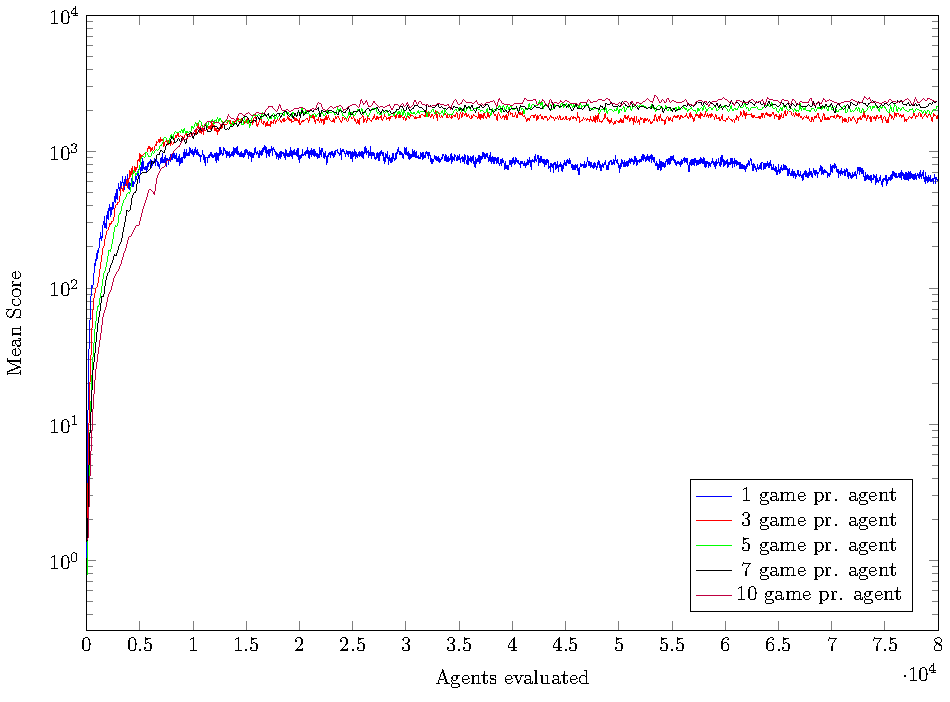
\includegraphics[width=\textwidth]{data/cma_population_offspring/12x_split/linear_l12_o6/mean/PlotFile.pdf}
    \end{subfigure}
    \begin{subfigure}[b]{0.49\textwidth}
    	\caption{Population size 12, Parent size 1,\\SUPERLINEAR recombination}
        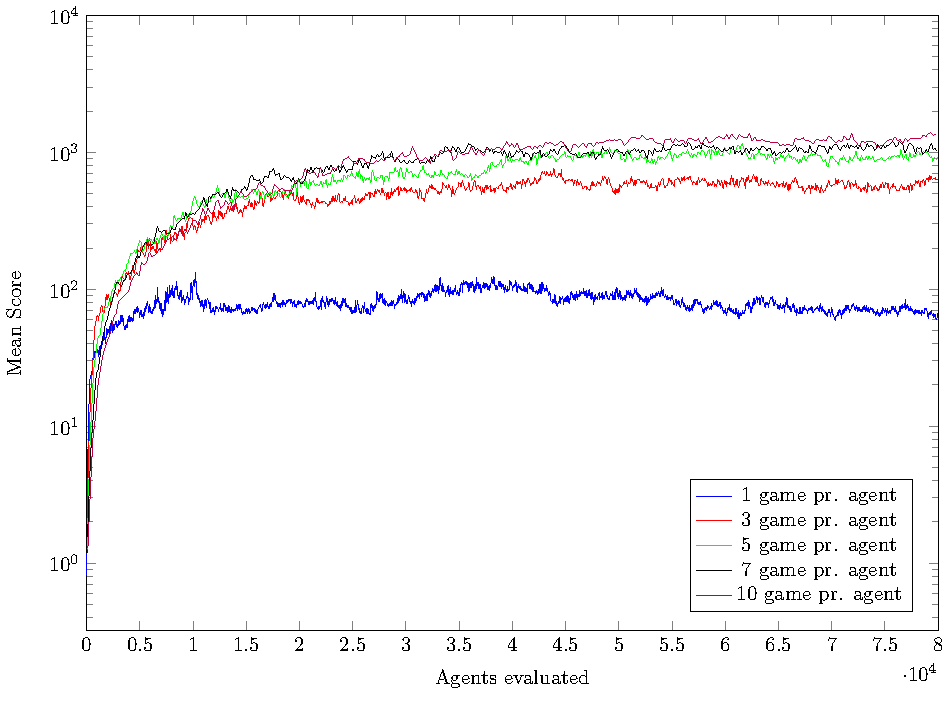
\includegraphics[width=\textwidth]{data/cma_population_offspring/12x_split/superlinear_l12_o1/mean/PlotFile.pdf}
    \end{subfigure}
    \begin{subfigure}[b]{0.49\textwidth}
    	\caption{Population size 12, Parent size 6,\\SUPERLINEAR recombination}
        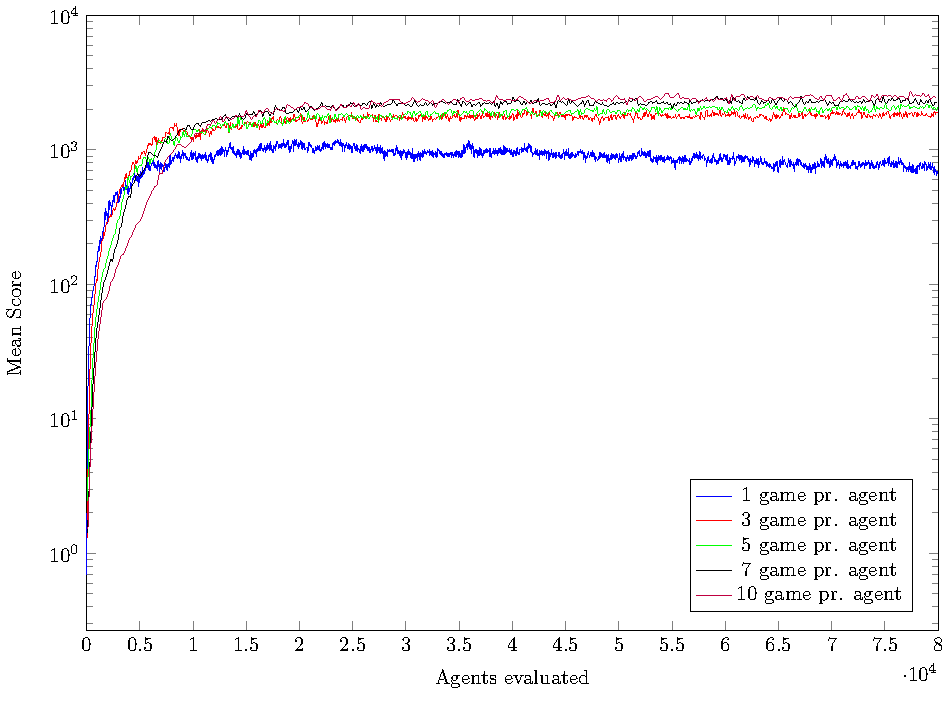
\includegraphics[width=\textwidth]{data/cma_population_offspring/12x_split/superlinear_l12_o6/mean/PlotFile.pdf}
    \end{subfigure}
    
    \caption{Mean results for population size 12 with variating recombination}
\end{figure}

\begin{figure}
    \centering
    \captionsetup[subfigure]{justification=centering}
    \begin{subfigure}[b]{0.49\textwidth}
    	\centering
        \caption{Population size 22, Parent size 2,\\EQUAL recombination}
        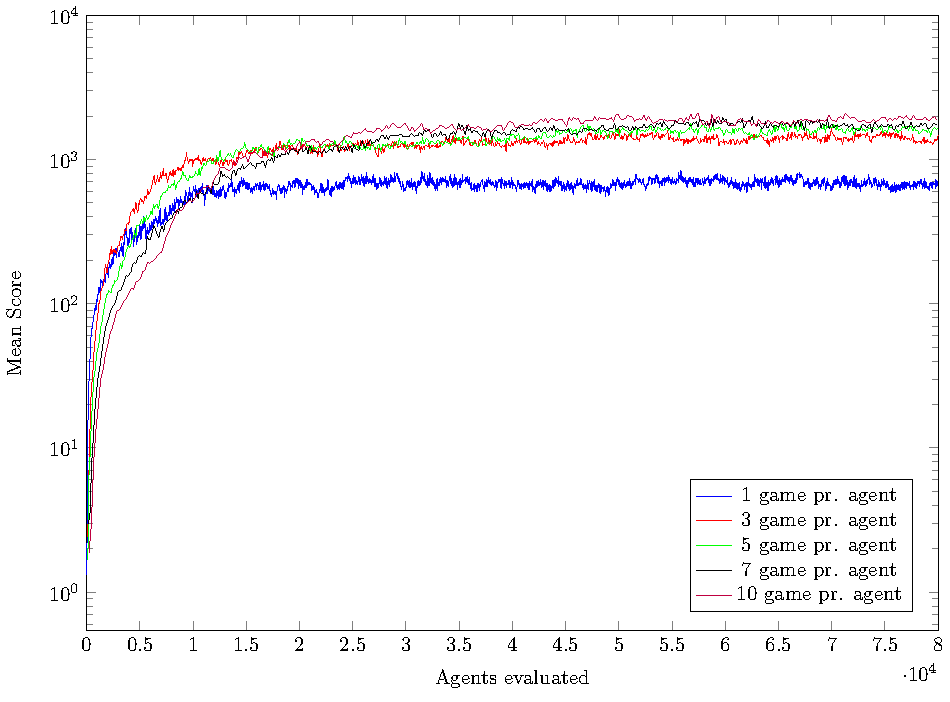
\includegraphics[width=\textwidth]{data/cma_population_offspring/22x_split/equal_l22_o2/mean/PlotFile.pdf}
    \end{subfigure} 
    \begin{subfigure}[b]{0.49\textwidth}
    	\centering
    	\caption{Population size 22, Parent size 5,\\EQUAL recombination}
        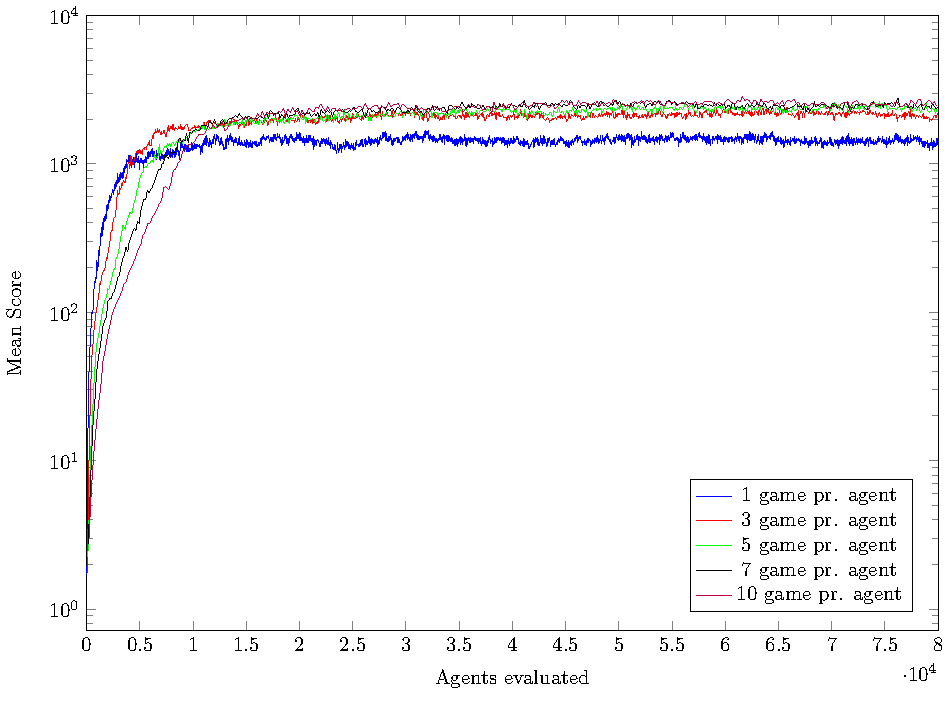
\includegraphics[width=\textwidth]{data/cma_population_offspring/22x_split/equal_l22_o5/mean/PlotFile.pdf}
    \end{subfigure}
    \begin{subfigure}[b]{0.49\textwidth}
    	\centering
    	\caption{Population size 22, Parent size 2,\\LINEAR recombination}
        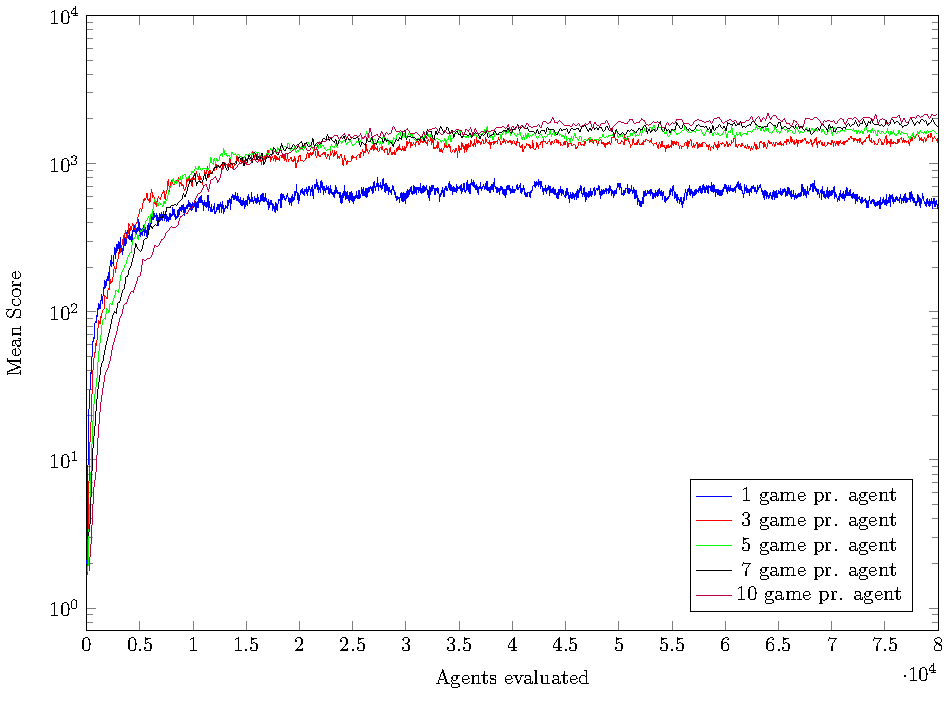
\includegraphics[width=\textwidth]{data/cma_population_offspring/22x_split/linear_l22_o2/mean/PlotFile.pdf}
    \end{subfigure}
    \begin{subfigure}[b]{0.49\textwidth}
    	\centering
    	\caption{Population size 22, Parent size 11,\\LINEAR recombination}
        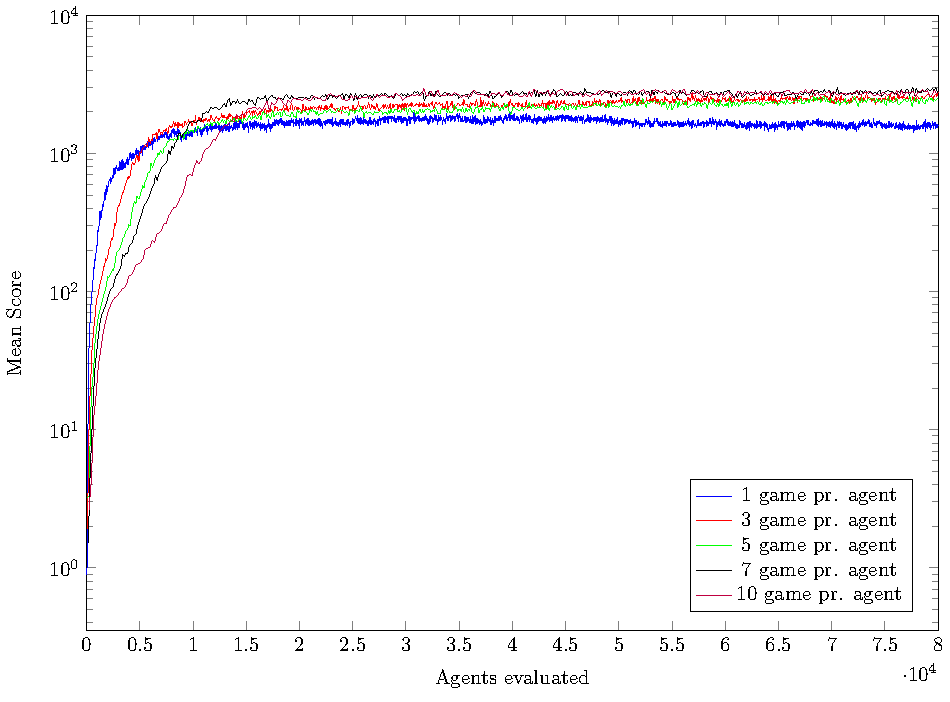
\includegraphics[width=\textwidth]{data/cma_population_offspring/22x_split/linear_l22_o11/mean/PlotFile.pdf}
    \end{subfigure}
    \begin{subfigure}[b]{0.49\textwidth}
    	\centering
    	\caption{Population size 22, Parent size 2,\\SUPERLINEAR recombination}
        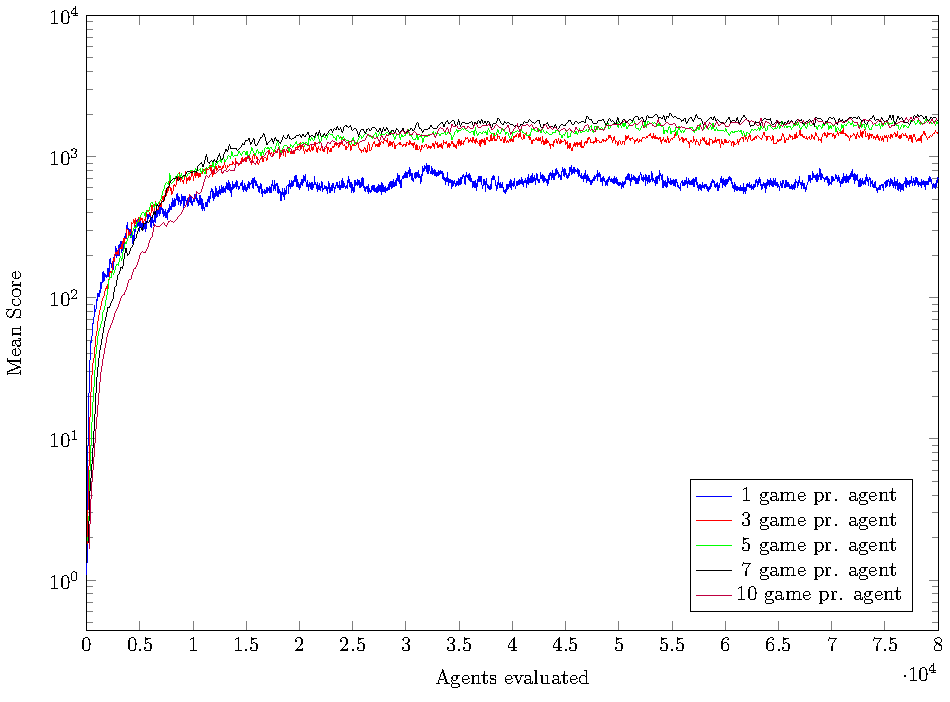
\includegraphics[width=\textwidth]{data/cma_population_offspring/22x_split/superlinear_l22_o2/mean/PlotFile.pdf}
    \end{subfigure}
    \begin{subfigure}[b]{0.49\textwidth}
    	\centering
    	\caption{Population size 22, Parent size 11,\\SUPERLINEAR recombination}
        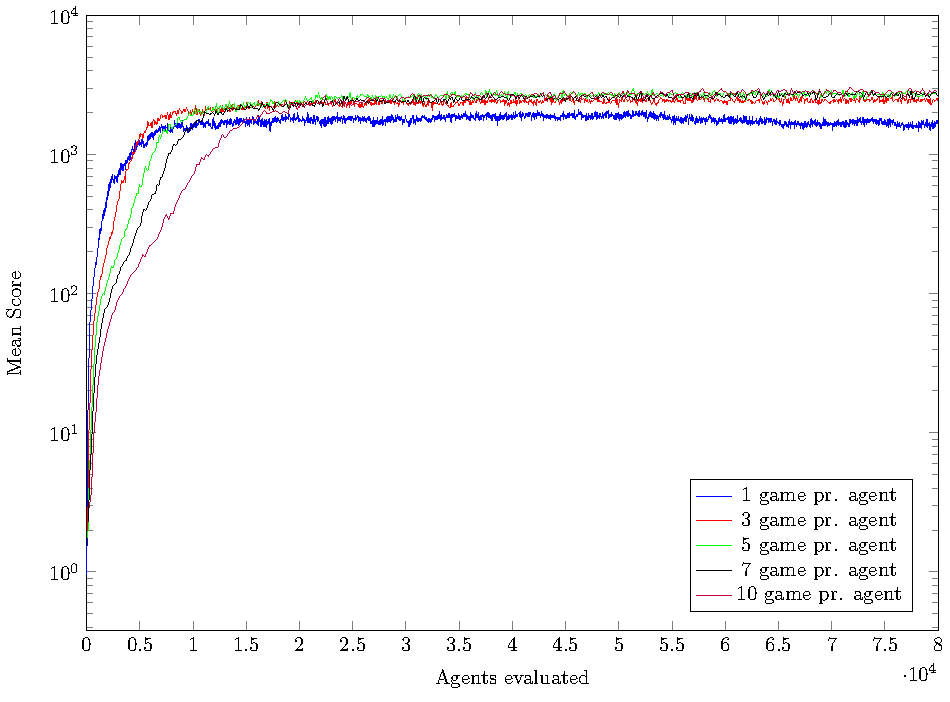
\includegraphics[width=\textwidth]{data/cma_population_offspring/22x_split/superlinear_l22_o11/mean/PlotFile.pdf}
    \end{subfigure}
    
    \caption{Mean results for population size 22 with variating recombination}
\end{figure}

\begin{figure}
    \centering
    \captionsetup[subfigure]{justification=centering}
    \begin{subfigure}[b]{0.49\textwidth}
    	\centering
        \caption{Population size 50, Parent size 5,\\EQUAL recombination}
        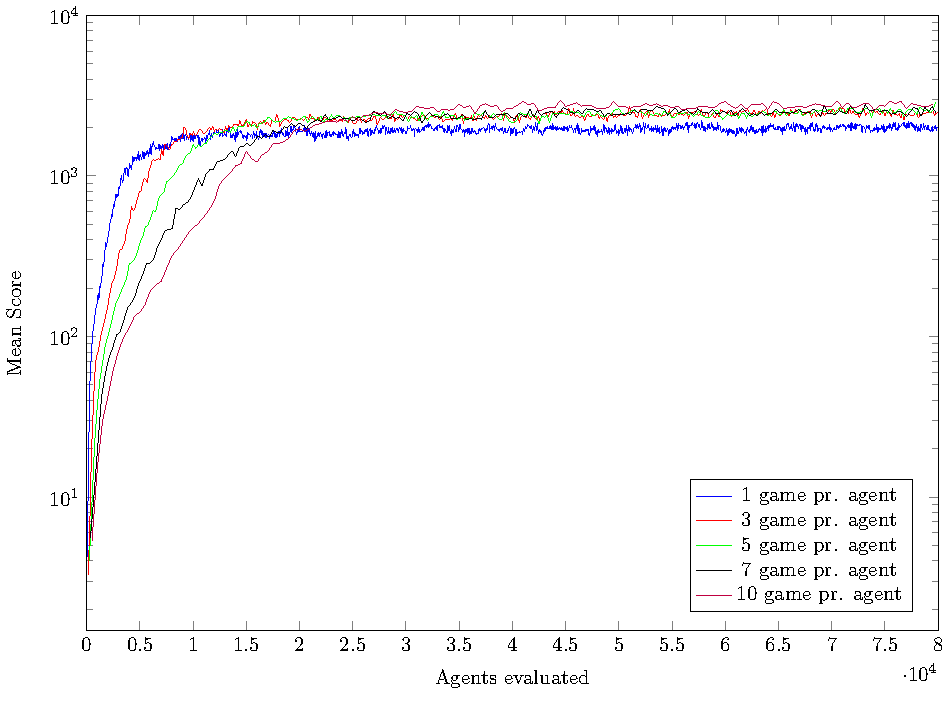
\includegraphics[width=\textwidth]{data/cma_population_offspring/50x_split/equal_l50_o5/mean/PlotFile.pdf}
    \end{subfigure} 
    \begin{subfigure}[b]{0.49\textwidth}
    	\centering
    	\caption{Population size 50, Parent size 12,\\EQUAL recombination}
        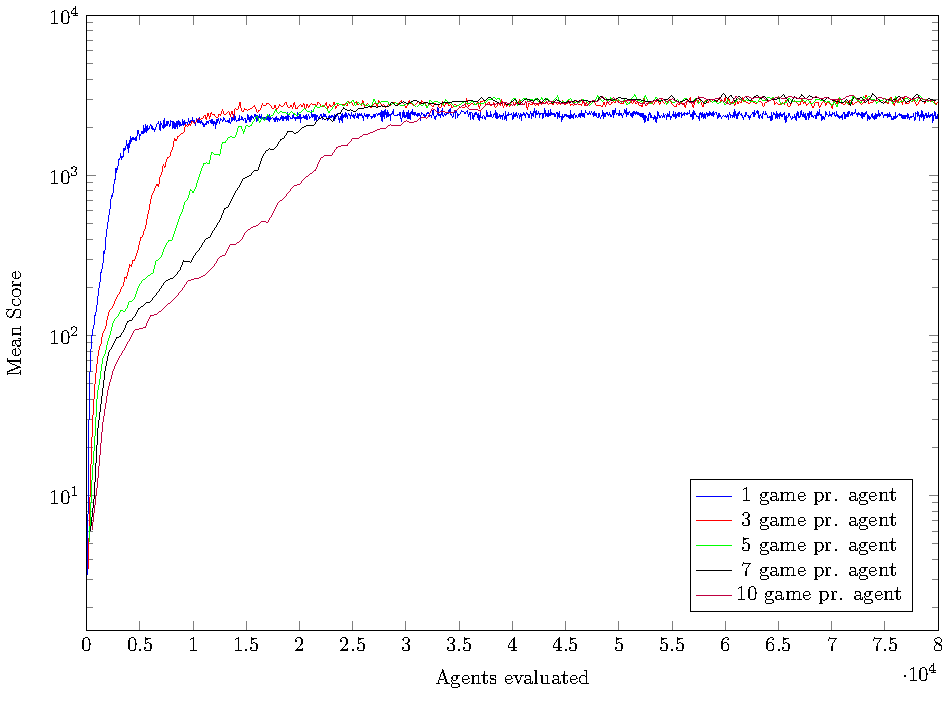
\includegraphics[width=\textwidth]{data/cma_population_offspring/50x_split/equal_l50_o12/mean/PlotFile.pdf}
    \end{subfigure}
    \begin{subfigure}[b]{0.49\textwidth}
    	\centering
    	\caption{Population size 50, Parent size 5,\\LINEAR recombination}
        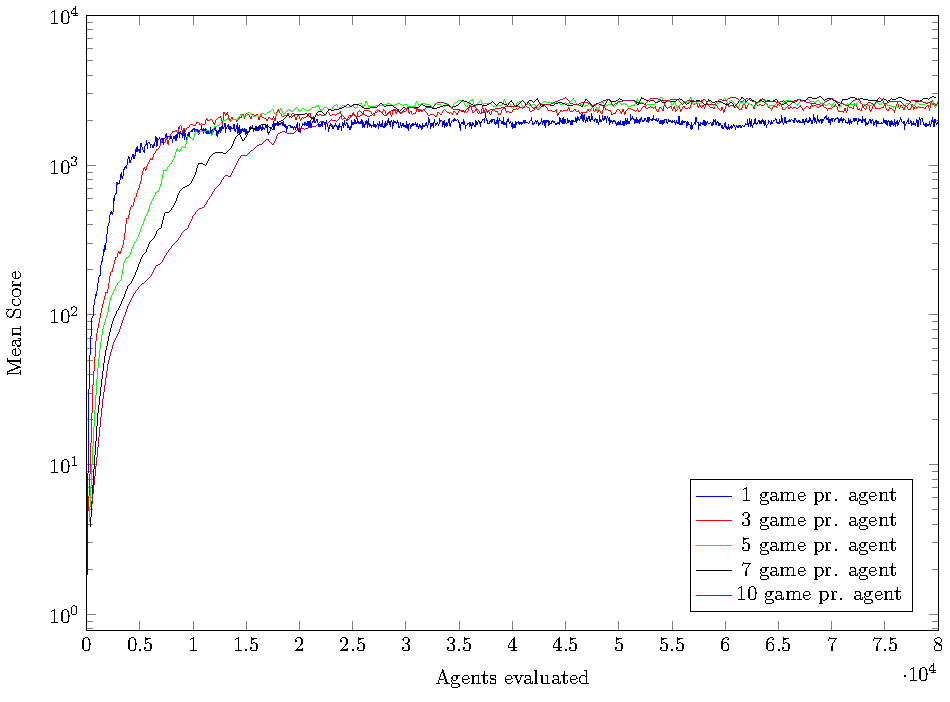
\includegraphics[width=\textwidth]{data/cma_population_offspring/50x_split/linear_l50_o5/mean/PlotFile.pdf}
    \end{subfigure}
    \begin{subfigure}[b]{0.49\textwidth}
    	\centering
    	\caption{Population size 50, Parent size 25,\\LINEAR recombination}
        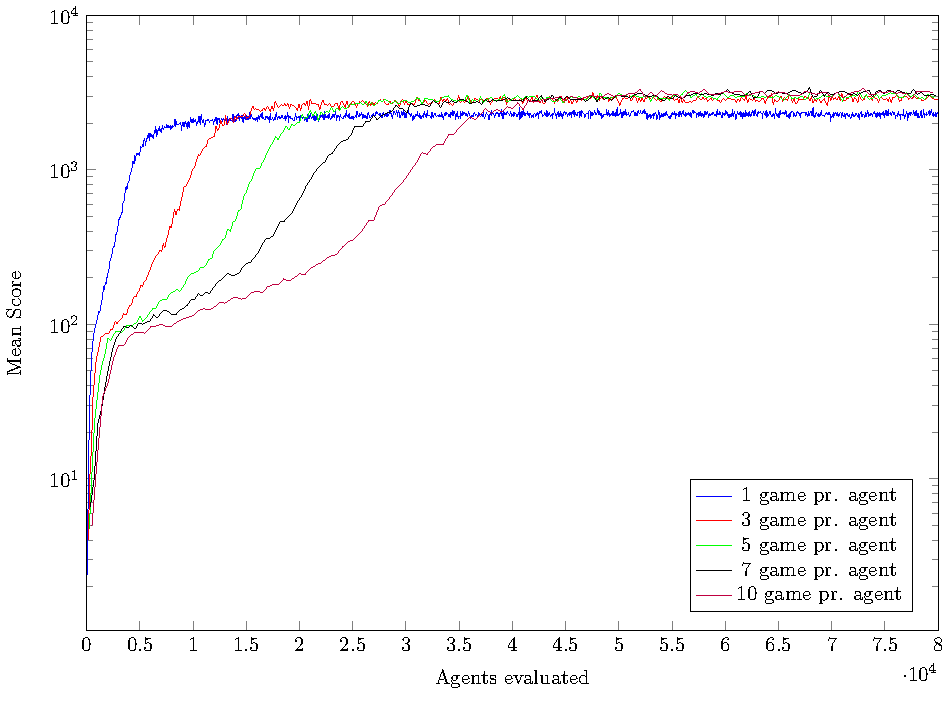
\includegraphics[width=\textwidth]{data/cma_population_offspring/50x_split/linear_l50_o25/mean/PlotFile.pdf}
    \end{subfigure}
    \begin{subfigure}[b]{0.49\textwidth}
    	\centering
    	\caption{Population size 50, Parent size 5,\\SUPERLINEAR recombination}
        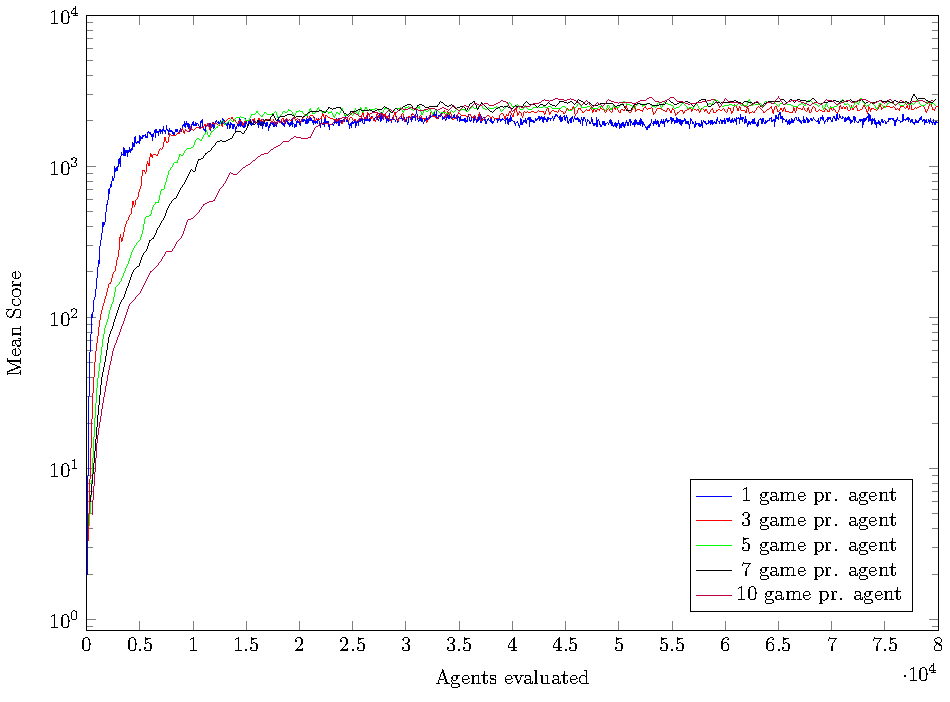
\includegraphics[width=\textwidth]{data/cma_population_offspring/50x_split/superlinear_l50_o5/mean/PlotFile.pdf}
    \end{subfigure}
    \begin{subfigure}[b]{0.49\textwidth}
    	\centering
    	\caption{Population size 50, Parent size 25,\\SUPERLINEAR recombination}
        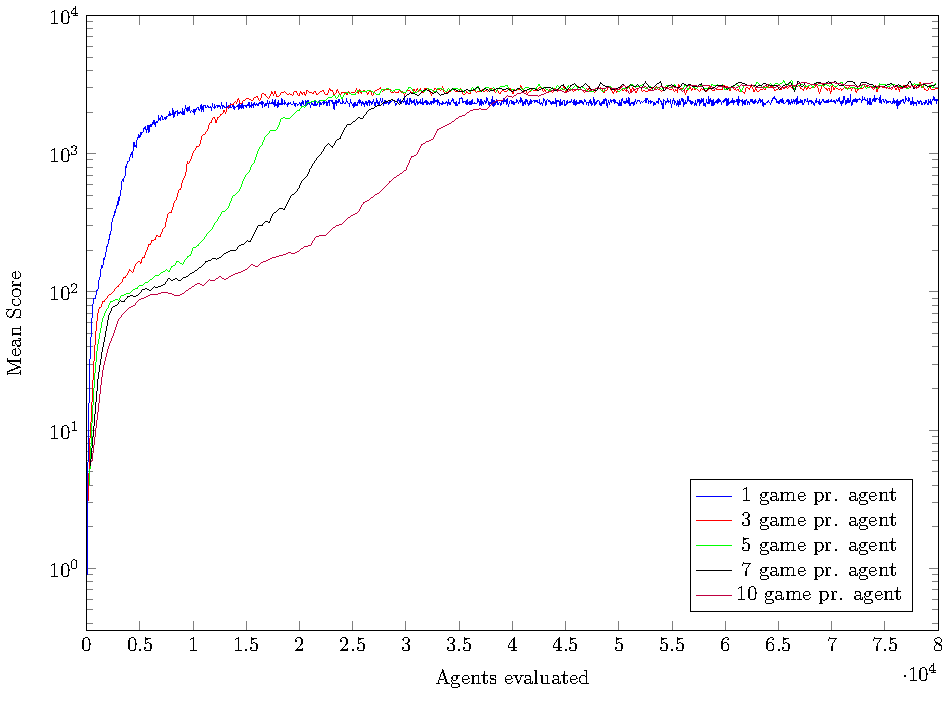
\includegraphics[width=\textwidth]{data/cma_population_offspring/50x_split/superlinear_l50_o25/mean/PlotFile.pdf}
    \end{subfigure}
    
    \caption{Mean results for population size 50 with variating recombination}
\end{figure}

\begin{figure}
    \centering
    \captionsetup[subfigure]{justification=centering}
    \begin{subfigure}[b]{0.49\textwidth}
    	\centering
        \caption{Population size 100, Parent size 10,\\EQUAL recombination}
        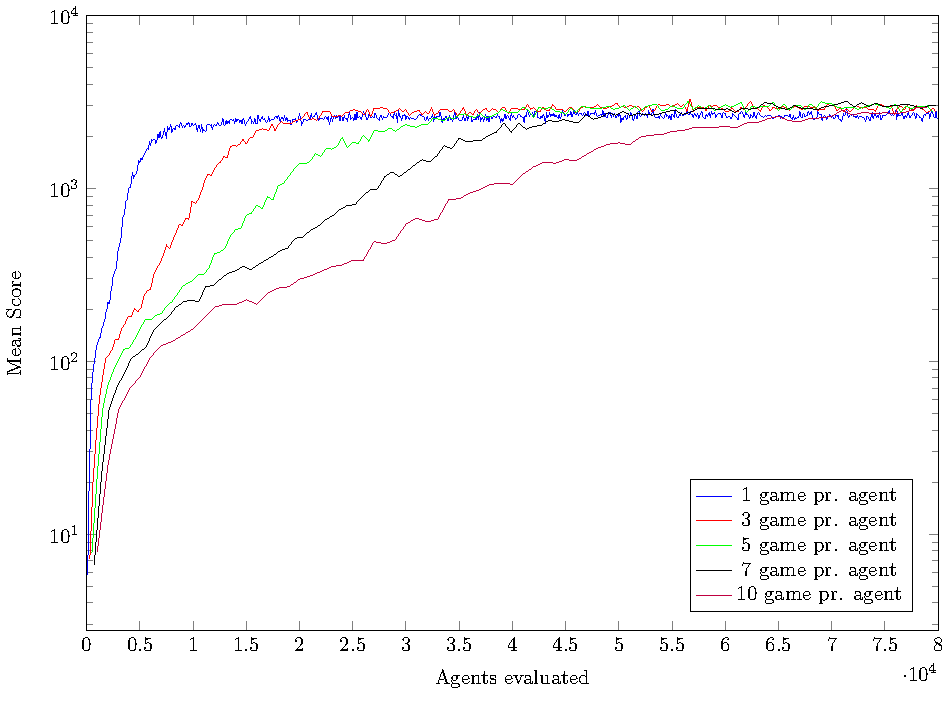
\includegraphics[width=\textwidth]{data/cma_population_offspring/100x_split/equal_l100_o10/mean/PlotFile.pdf}
    \end{subfigure} 
    \begin{subfigure}[b]{0.49\textwidth}
    	\centering
    	\caption{Population size 100, Parent size 25,\\EQUAL recombination}
        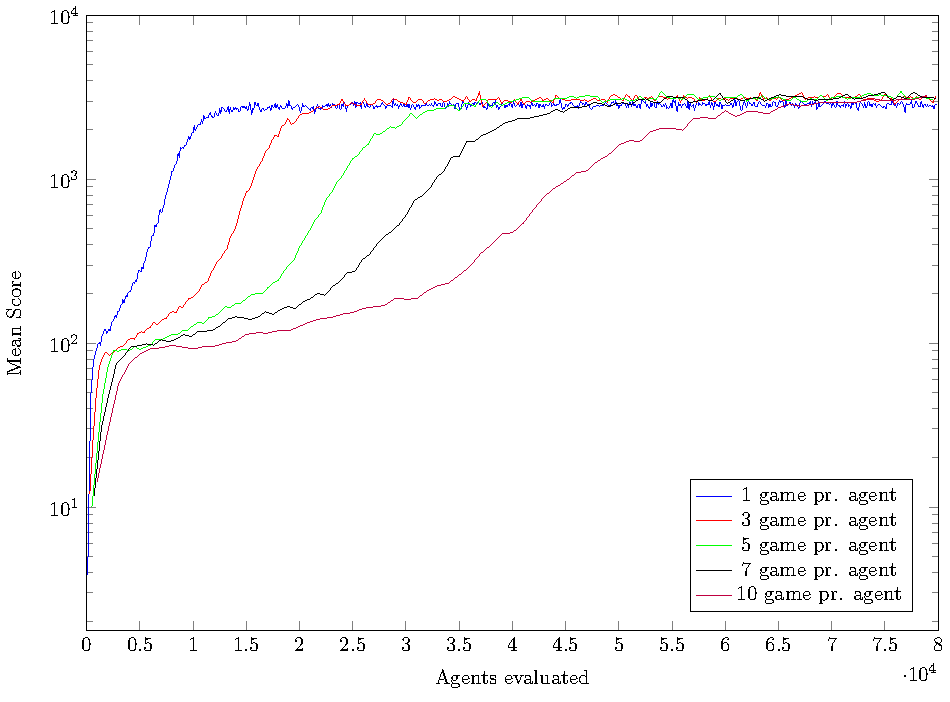
\includegraphics[width=\textwidth]{data/cma_population_offspring/100x_split/equal_l100_o25/mean/PlotFile.pdf}
    \end{subfigure}
    \begin{subfigure}[b]{0.49\textwidth}
    	\centering
    	\caption{Population size 100, Parent size 10,\\LINEAR recombination}
        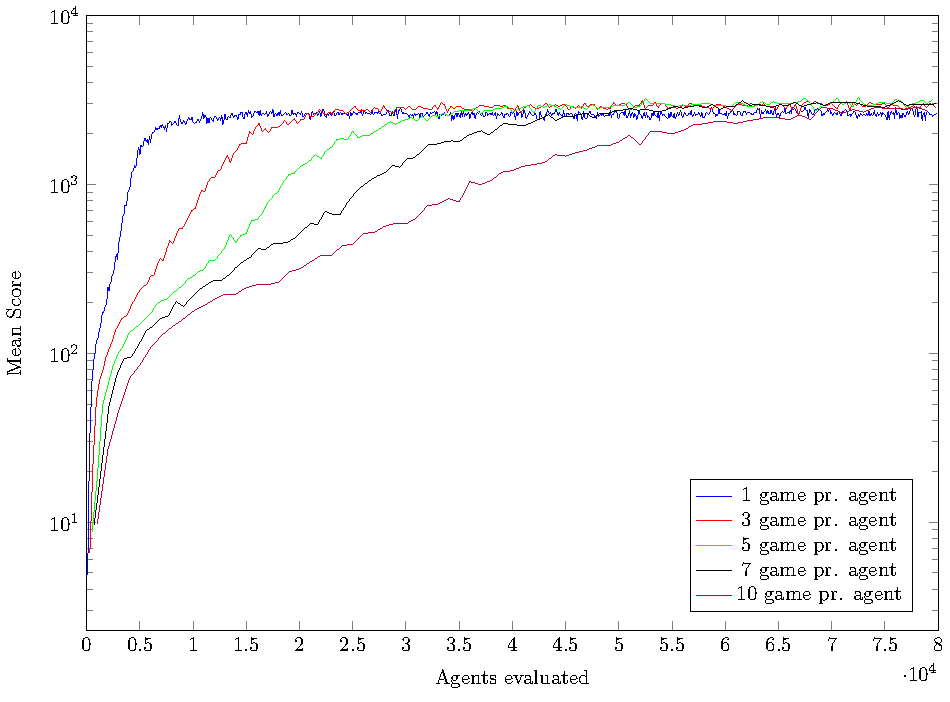
\includegraphics[width=\textwidth]{data/cma_population_offspring/100x_split/linear_l100_o10/mean/PlotFile.pdf}
    \end{subfigure}
    \begin{subfigure}[b]{0.49\textwidth}
    	\centering
    	\caption{Population size 100, Parent size 50,\\LINEAR recombination}
        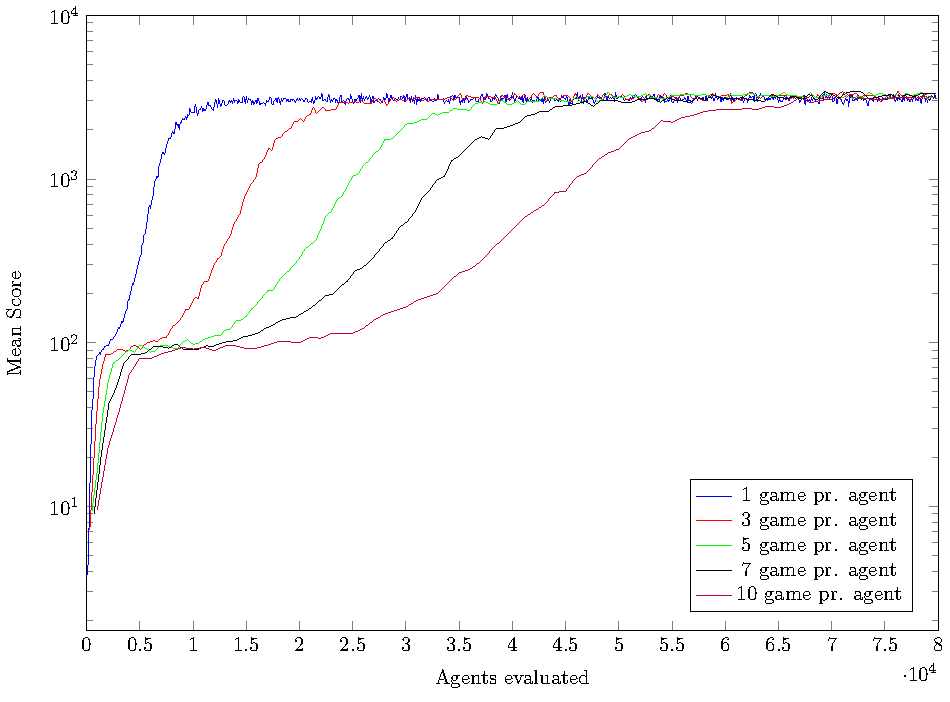
\includegraphics[width=\textwidth]{data/cma_population_offspring/100x_split/linear_l100_o50/mean/PlotFile.pdf}
    \end{subfigure}
    \begin{subfigure}[b]{0.49\textwidth}
    	\centering
    	\caption{Population size 100, Parent size 10,\\SUPERLINEAR recombination}
        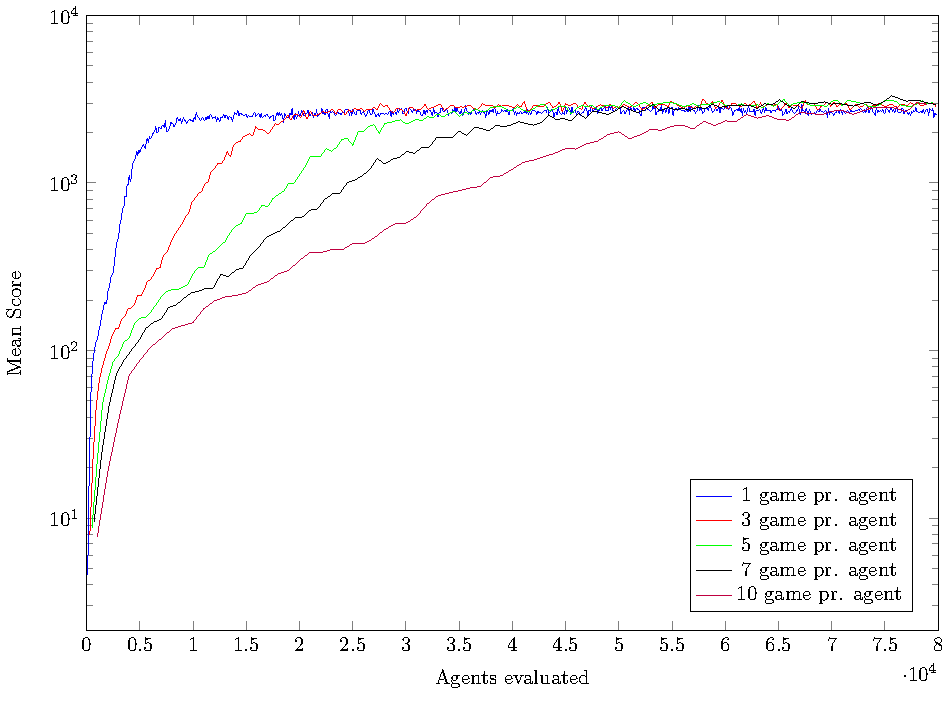
\includegraphics[width=\textwidth]{data/cma_population_offspring/100x_split/superlinear_l100_o10/mean/PlotFile.pdf}
    \end{subfigure}
    \begin{subfigure}[b]{0.49\textwidth}
    	\centering
    	\caption{Population size 100, Parent size 50,\\SUPERLINEAR recombination}
        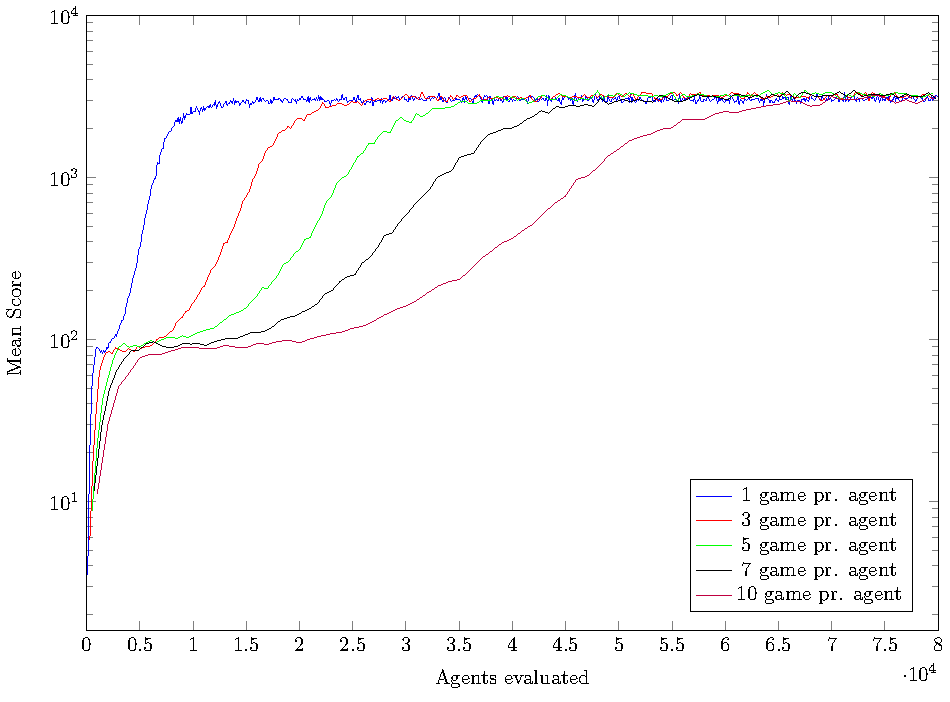
\includegraphics[width=\textwidth]{data/cma_population_offspring/100x_split/superlinear_l100_o50/mean/PlotFile.pdf}
    \end{subfigure}
    
    \caption{Mean results for population size 100 with variating recombination}
\end{figure}

\clearpage

\begin{table}[H]
\centering
\small
\begin{tabular}{c c c c r r r r}
Population & Parent & Recombination & Games per Agent & mean & Q1 & Q2 & Q3\\
\hline
$12$ & $1$ & EQUAL & 1 & $86.998$ & $53.557$ & $63.417$ & $111.313$\\
$12$ & $1$ & EQUAL & 3 & $458.616$ & $256.637$ & $349.033$ & $576.899$\\
$12$ & $1$ & EQUAL & 5 & $1089.245$ & $850.220$ & $1104.535$ & $1299.039$\\
$12$ & $1$ & EQUAL & 7 & $1081.248$ & $918.049$ & $1089.400$ & $1248.619$\\
\hdashline
$12$ & $1$ & EQUAL & 10 & $1134.339$ & $863.523$ & $1061.050$ & $1297.359$\\
\hdashline
$12$ & $1$ & LINEAR & 1 & $76.228$ & $45.587$ & $53.917$ & $74.353$\\
$12$ & $1$ & LINEAR & 3 & $717.883$ & $380.890$ & $556.950$ & $878.597$\\
$12$ & $1$ & LINEAR & 5 & $720.393$ & $503.130$ & $708.484$ & $893.517$\\
$12$ & $1$ & LINEAR & 7 & $1043.547$ & $732.367$ & $969.217$ & $1234.040$\\
\hdashline
$12$ & $1$ & LINEAR & 10 & $1276.041$ & $1135.609$ & $1196.120$ & $1502.029$\\
\hdashline
$12$ & $1$ & SUPERLINEAR & 1 & $64.211$ & $45.687$ & $64.483$ & $78.090$\\
$12$ & $1$ & SUPERLINEAR & 3 & $646.760$ & $429.043$ & $661.817$ & $860.470$\\
$12$ & $1$ & SUPERLINEAR & 5 & $925.410$ & $726.360$ & $948.300$ & $1158.021$\\
$12$ & $1$ & SUPERLINEAR & 7 & $1034.002$ & $792.567$ & $924.350$ & $1269.131$\\
\hdashline
$12$ & $1$ & SUPERLINEAR & 10 & $1401.300$ & $1194.430$ & $1440.500$ & $1569.012$\\
\hdashline
\end{tabular}
\caption{Population size 12, Parent size 1 - "Cross Entropy"-inspired configuration}
\end{table}

\begin{table}[H]
\centering
\small
\begin{tabular}{c c c c r r r r}
Population & Parent & Recombination & Games per Agent & mean & Q1 & Q2 & Q3\\
\hline
$12$ & $3$ & EQUAL & 1 & $461.762$ & $266.047$ & $408.034$ & $639.013$\\
$12$ & $3$ & EQUAL & 3 & $1364.176$ & $1199.310$ & $1438.880$ & $1579.560$\\
$12$ & $3$ & EQUAL & 5 & $1754.634$ & $1464.239$ & $1621.035$ & $1945.010$\\
$12$ & $3$ & EQUAL & 7 & $1884.765$ & $1614.661$ & $1800.485$ & $2156.972$\\
\hdashline
$12$ & $3$ & EQUAL & 10 & $1940.783$ & $1566.721$ & $1913.415$ & $2210.251$\\
\hdashline
$12$ & $6$ & LINEAR & 1 & $626.867$ & $447.440$ & $538.150$ & $724.913$\\
$12$ & $6$ & LINEAR & 3 & $1844.453$ & $1568.829$ & $1831.265$ & $2227.479$\\
$12$ & $6$ & LINEAR & 5 & $2148.853$ & $1846.459$ & $2118.335$ & $2588.010$\\
$12$ & $6$ & LINEAR & 7 & $2144.345$ & $1860.340$ & $2160.900$ & $2428.348$\\
\hdashline
$12$ & $6$ & LINEAR & 10 & $2365.089$ & $2072.719$ & $2263.665$ & $2637.732$\\
\hdashline
$12$ & $6$ & SUPERLINEAR & 1 & $669.005$ & $506.817$ & $648.167$ & $836.377$\\
$12$ & $6$ & SUPERLINEAR & 3 & $1901.814$ & $1572.260$ & $1932.515$ & $2151.189$\\
$12$ & $6$ & SUPERLINEAR & 5 & $2098.654$ & $1965.472$ & $2115.250$ & $2453.069$\\
$12$ & $6$ & SUPERLINEAR & 7 & $2402.888$ & $2055.329$ & $2387.700$ & $2635.870$\\
\hdashline
$12$ & $6$ & SUPERLINEAR & 10 & $2472.293$ & $2194.049$ & $2430.780$ & $2709.040$\\
\hdashline
\end{tabular}
\caption{Population size 12, Parent size 3/6 - CMA configuration}
\end{table}


\begin{table}[H]
\centering
\small
\begin{tabular}{c c c c r r r r}
Population & Parent & Recombination & Games per Agent & mean & Q1 & Q2 & Q3\\
\hline
$22$ & $2$ & EQUAL & 1 & $684.551$ & $429.890$ & $597.534$ & $877.150$\\
$22$ & $2$ & EQUAL & 3 & $1473.504$ & $1197.290$ & $1490.865$ & $1713.091$\\
$22$ & $2$ & EQUAL & 5 & $1648.777$ & $1425.150$ & $1630.535$ & $1826.372$\\
$22$ & $2$ & EQUAL & 7 & $1762.786$ & $1521.832$ & $1769.180$ & $2033.799$\\
\hdashline
$22$ & $2$ & EQUAL & 10 & $1895.305$ & $1630.891$ & $1849.75$ & $2043.442$\\
\hdashline
$22$ & $2$ & LINEAR & 1 & $513.271$ & $398.023$ & $524.850$ & $589.467$\\
$22$ & $2$ & LINEAR & 3 & $1374.423$ & $1082.859$ & $1255.985$ & $1561.119$\\
$22$ & $2$ & LINEAR & 5 & $1607.568$ & $1513.389$ & $1656.465$ & $1791.069$\\
$22$ & $2$ & LINEAR & 7 & $1770.294$ & $1538.900$ & $1691.165$ & $1881.590$\\
\hdashline
$22$ & $2$ & LINEAR & 10 & $2158.396$ & $1966.351$ & $2085.235$ & $2162.541$\\
\hdashline
$22$ & $2$ & SUPERLINEAR & 1 & $698.811$ & $359.367$ & $622.467$ & $937.423$\\
$22$ & $2$ & SUPERLINEAR & 3 & $1447.704$ & $1281.119$ & $1452.680$ & $1640.468$\\
$22$ & $2$ & SUPERLINEAR & 5 & $1714.875$ & $1362.931$ & $1733.230$ & $2023.590$\\
\hdashline
$22$ & $2$ & SUPERLINEAR & 7 & $1783.623$ & $1603.389$ & $1720.335$ & $1937.749$\\
\hdashline
$22$ & $2$ & SUPERLINEAR & 10 & $1859.642$ & $1636.870$ & $1915.650$ & $2208.830$\\
\end{tabular}
\caption{Population size 22, Parent size 2 - "Cross Entropy"-inspired configuration}
\end{table}


\begin{table}[H]
\centering
\small
\begin{tabular}{c c c c r r r r}
Population & Parent & Recombination & Games per Agent & mean & Q1 & Q2 & Q3\\
\hline
$22$ & $5$ & EQUAL & 1 & $1411.458$ & $1207.060$ & $1528.050$ & $1707.590$\\
$22$ & $5$ & EQUAL & 3 & $2209.730$ & $2129.521$ & $2213.285$ & $2471.751$\\
$22$ & $5$ & EQUAL & 5 & $2274.419$ & $1933.249$ & $2187.800$ & $2570.399$\\
$22$ & $5$ & EQUAL & 7 & $2386.088$ & $2112.841$ & $2328.500$ & $2573.261$\\
\hdashline
$22$ & $5$ & EQUAL & 10 & $2462.409$ & $2277.180$ & $2418.100$ & $2600.411$\\
\hdashline
$22$ & $11$ & LINEAR & 1 & $1604.434$ & $1181.603$ & $1549.735$ & $1678.111$\\
$22$ & $11$ & LINEAR & 3 & $2774.378$ & $2460.992$ & $2594.900$ & $3030.310$\\
$22$ & $11$ & LINEAR & 5 & $2530.796$ & $2382.050$ & $2658.915$ & $2990.851$\\
\hdashline
$22$ & $11$ & LINEAR & 7 & $2763.353$ & $2597.450$ & $2705.080$ & $3000.242$\\
\hdashline
$22$ & $11$ & LINEAR & 10 & $2707.983$ & $2146.209$ & $2800.435$ & $3273.401$\\
$22$ & $11$ & SUPERLINEAR & 1 & $1666.214$ & $1447.430$ & $1660.900$ & $1856.908$\\
$22$ & $11$ & SUPERLINEAR & 3 & $2581.119$ & $2306.02$ & $2548.380$ & $2759.428$\\
$22$ & $11$ & SUPERLINEAR & 5 & $2635.429$ & $2409.620$ & $2574.785$ & $2863.849$\\
$22$ & $11$ & SUPERLINEAR & 7 & $2661.638$ & $2411.232$ & $2575.030$ & $2945.200$\\
\hdashline
$22$ & $11$ & SUPERLINEAR & 10 & $2849.220$ & $2500.231$ & $2835.450$ & $3143.121$\\
\hdashline
\end{tabular}
\caption{Population size 22, Parent size 5/11 - CMA configuration}
\end{table}


\begin{table}[H]
\centering
\small
\begin{tabular}{c c c c r r r r}
Population & Parent & Recombination & Games per Agent & mean & Q1 & Q2 & Q3\\
\hline
$50$ & $5$ & EQUAL & 1 & $1999.620$ & $1789.150$ & $1902.020$ & $2161.948$\\
$50$ & $5$ & EQUAL & 3 & $2471.173$ & $2178.651$ & $2389.070$ & $2660.220$\\
$50$ & $5$ & EQUAL & 5 & $2849.482$ & $2459.460$ & $2875.835$ & $3276.190$\\
$50$ & $5$ & EQUAL & 7 & $2466.801$ & $2355.349$ & $2517.335$ & $2644.751$\\
\hdashline
$50$ & $5$ & EQUAL & 10 & $2801.923$ & $2479.088$ & $2915.980$ & $3081.018$\\
\hdashline
$50$ & $5$ & LINEAR & 1 & $1931.703$ & $1659.412$ & $1885.150$ & $2130.479$\\
$50$ & $5$ & LINEAR & 3 & $2612.345$ & $2380.759$ & $2529.150$ & $2796.729$\\
$50$ & $5$ & LINEAR & 5 & $2410.633$ & $2067.111$ & $2357.830$ & $2675.572$\\
\hdashline
$50$ & $5$ & LINEAR & 7 & $2842.090$ & $2497.952$ & $2922.965$ & $3136.509$\\
\hdashline
$50$ & $5$ & LINEAR & 10 & $2696.952$ & $2518.290$ & $2678.400$ & $2923.010$\\
$50$ & $5$ & SUPERLINEAR & 1 & $1962.410$ & $1715.568$ & $1781.865$ & $2009.488$\\
$50$ & $5$ & SUPERLINEAR & 3 & $2493.884$ & $2220.200$ & $2398.230$ & $2762.609$\\
$50$ & $5$ & SUPERLINEAR & 5 & $2541.065$ & $2268.881$ & $2593.150$ & $2974.558$\\
$50$ & $5$ & SUPERLINEAR & 7 & $2647.412$ & $2448.010$ & $2745.400$ & $3058.870$\\
\hdashline
$50$ & $5$ & SUPERLINEAR & 10 & $2757.388$ & $2357.062$ & $2886.950$ & $3187.282$\\
\hdashline
\end{tabular}
\caption{Population size 50, Parent size 5 - "Cross Entropy"-inspired configuration}
\end{table}

\begin{table}[H]
\centering
\small
\begin{tabular}{c c c c r r r r}
Population & Parent & Recombination & Games per Agent & mean & Q1 & Q2 & Q3\\
\hline
$50$ & $12$ & EQUAL & 1 & $2395.091$ & $2095.030$ & $2442.485$ & $2778.160$\\
$50$ & $12$ & EQUAL & 3 & $2878.667$ & $2550.399$ & $2794.915$ & $3102.639$\\
$50$ & $12$ & EQUAL & 5 & $2760.846$ & $2509.000$ & $2695.450$ & $3006.988$\\
$50$ & $12$ & EQUAL & 7 & $2913.846$ & $2627.310$ & $2809.600$ & $3128.439$\\
\hdashline
$50$ & $12$ & EQUAL & 10 & $2957.794$ & $2636.478$ & $2843.380$ & $3222.420$\\
\hdashline
$50$ & $25$ & LINEAR & 1 & $2355.564$ & $2262.991$ & $2543.665$ & $2752.431$\\
$50$ & $25$ & LINEAR & 3 & $2857.170$ & $2464.251$ & $2830.765$ & $3209.929$\\
$50$ & $25$ & LINEAR & 5 & $3036.881$ & $2807.050$ & $3095.300$ & $3416.750$\\
$50$ & $25$ & LINEAR & 7 & $3043.399$ & $2821.049$ & $3099.235$ & $3239.032$\\
\hdashline
$50$ & $25$ & LINEAR & 10 & $3167.873$ & $2941.590$ & $3130.385$ & $3415.520$\\
\hdashline
$50$ & $25$ & SUPERLINEAR & 1 & $2418.057$ & $2352.851$ & $2553.465$ & $2718.759$\\
$50$ & $25$ & SUPERLINEAR & 3 & $2958.686$ & $2715.579$ & $2941.800$ & $3173.361$\\
\hdashline
$50$ & $25$ & SUPERLINEAR & 5 & $3211.658$ & $2889.689$ & $3305.485$ & $3694.480$\\
\hdashline
$50$ & $25$ & SUPERLINEAR & 7 & $3147.611$ & $2799.510$ & $3123.550$ & $3457.999$\\
$50$ & $25$ & SUPERLINEAR & 10 & $3265.516$ & $2928.771$ & $3162.250$ & $3389.121$\\
\end{tabular}
\caption{Population size 50, Parent size 12/25 - CMA configuration}
\end{table}


\begin{table}[H]
\centering
\small
\begin{tabular}{c c c c r r r r}
Population & Parent & Recombination & Games per Agent & mean & Q1 & Q2 & Q3\\
\hline
$100$ & $10$ & EQUAL & 1 & $2528.158$ & $2380.122$ & $2680.785$ & $2782.850$\\
$100$ & $10$ & EQUAL & 3 & $2763.118$ & $2488.878$ & $2696.685$ & $2962.190$\\
$100$ & $10$ & EQUAL & 5 & $2783.246$ & $2399.949$ & $2693.285$ & $2900.391$\\
\hdashline
$100$ & $10$ & EQUAL & 7 & $3016.342$ & $2835.049$ & $2985.150$ & $3292.910$\\
\hdashline
$100$ & $10$ & EQUAL & 10 & $2940.037$ & $2703.859$ & $2920.615$ & $3216.410$\\
$100$ & $10$ & LINEAR & 1 & $2655.099$ & $2409.162$ & $2691.850$ & $2961.091$\\
$100$ & $10$ & LINEAR & 3 & $2823.674$ & $2526.560$ & $2792.500$ & $2974.549$\\
\hdashline
$100$ & $10$ & LINEAR & 5 & $3204.395$ & $2928.050$ & $3248.515$ & $3371.008$\\
\hdashline
$100$ & $10$ & LINEAR & 7 & $2993.126$ & $2639.021$ & $3031.065$ & $3277.642$\\
$100$ & $10$ & LINEAR & 10 & $2726.273$ & $2402.502$ & $2748.535$ & $3009.198$\\
$100$ & $10$ & SUPERLINEAR & 1 & $2571.936$ & $2211.051$ & $2634.850$ & $2811.190$\\
$100$ & $10$ & SUPERLINEAR & 3 & $2853.959$ & $2552.749$ & $2870.600$ & $3005.292$\\
\hdashline
$100$ & $10$ & SUPERLINEAR & 5 & $3009.495$ & $2816.660$ & $2989.900$ & $3189.310$\\
\hdashline
$100$ & $10$ & SUPERLINEAR & 7 & $2935.614$ & $2540.342$ & $2887.085$ & $3232.508$\\
$100$ & $10$ & SUPERLINEAR & 10 & $2941.535$ & $2705.290$ & $2893.580$ & $3153.510$\\
\end{tabular}
\caption{Population size 100, Parent size 10 - "Cross Entropy"-inspired configuration}
\end{table}


\begin{table}[H]
\centering
\small
\begin{tabular}{c c c c r r r r}
Population & Parent & Recombination & Games per Agent & mean & Q1 & Q2 & Q3\\
\hline
$100$ & $25$ & EQUAL & 1 & $2885.131$ & $2565.572$ & $2886.735$ & $3231.600$\\
\hdashline
$100$ & $25$ & EQUAL & 3 & $3244.544$ & $2924.488$ & $3270.885$ & $3525.671$\\
\hdashline
$100$ & $25$ & EQUAL & 5 & $3065.143$ & $2773.848$ & $3032.830$ & $3347.358$\\
$100$ & $25$ & EQUAL & 7 & $3125.085$ & $2758.298$ & $3054.950$ & $3486.672$\\
$100$ & $25$ & EQUAL & 10 & $3258.533$ & $2976.271$ & $3144.750$ & $3598.868$\\
$100$ & $50$ & LINEAR & 1 & $3099.651$ & $2814.781$ & $3019.830$ & $3466.380$\\
$100$ & $50$ & LINEAR & 3 & $3125.019$ & $2706.618$ & $3087.815$ & $3368.681$\\
$100$ & $50$ & LINEAR & 5 & $3171.761$ & $2941.030$ & $3138.515$ & $3436.670$\\
\hdashline
$100$ & $50$ & LINEAR & 7 & $3322.076$ & $3160.098$ & $3289.370$ & $3537.850$\\
\hdashline
$100$ & $50$ & LINEAR & 10 & $3320.153$ & $3040.611$ & $3291.335$ & $3633.491$\\
$100$ & $50$ & SUPERLINEAR & 1 & $3162.245$ & $2815.099$ & $3093.050$ & $3482.748$\\
$100$ & $50$ & SUPERLINEAR & 3 & $3188.324$ & $2781.382$ & $3258.400$ & $3413.710$\\
\hdashline
$100$ & $50$ & SUPERLINEAR & 5 & $3304.119$ & $3004.140$ & $3226.235$ & $3679.359$\\
\hdashline
$100$ & $50$ & SUPERLINEAR & 7 & $3072.331$ & $2682.300$ & $2964.850$ & $3403.132$\\
$100$ & $50$ & SUPERLINEAR & 10 & $3106.917$ & $2914.349$ & $3162.250$ & $3324.970$\\
\end{tabular}
\caption{Population size 100, Parent size 25/50 - CMA configuration}
\end{table}

\clearpage

\begin{table}[H]
\centering
\small
\begin{tabular}{c c c c r r r r}
Population & Parent & Recombination & Games per Agent & mean & Q1 & Q2 & Q3\\
\hline
$12$ & $1$ & EQUAL & 10 & $1134.339$ & $863.523$ & $1061.050$ & $1297.359$\\
$12$ & $1$ & LINEAR & 10 & $1276.041$ & $1135.609$ & $1196.120$ & $1502.029$\\
$12$ & $1$ & SUPERLINEAR & 10 & $1401.300$ & $1194.430$ & $1440.500$ & $1569.012$\\
$12$ & $3$ & EQUAL & 10 & $1940.783$ & $1566.721$ & $1913.415$ & $2210.251$\\
$12$ & $6$ & LINEAR & 10 & $2365.089$ & $2072.719$ & $2263.665$ & $2637.732$\\
$12$ & $6$ & SUPERLINEAR & 10 & $2472.293$ & $2194.049$ & $2430.780$ & $2709.040$\\
\end{tabular}
\caption{Best performing configurations for population size 12}
\end{table}

\begin{figure}[H]
\centering
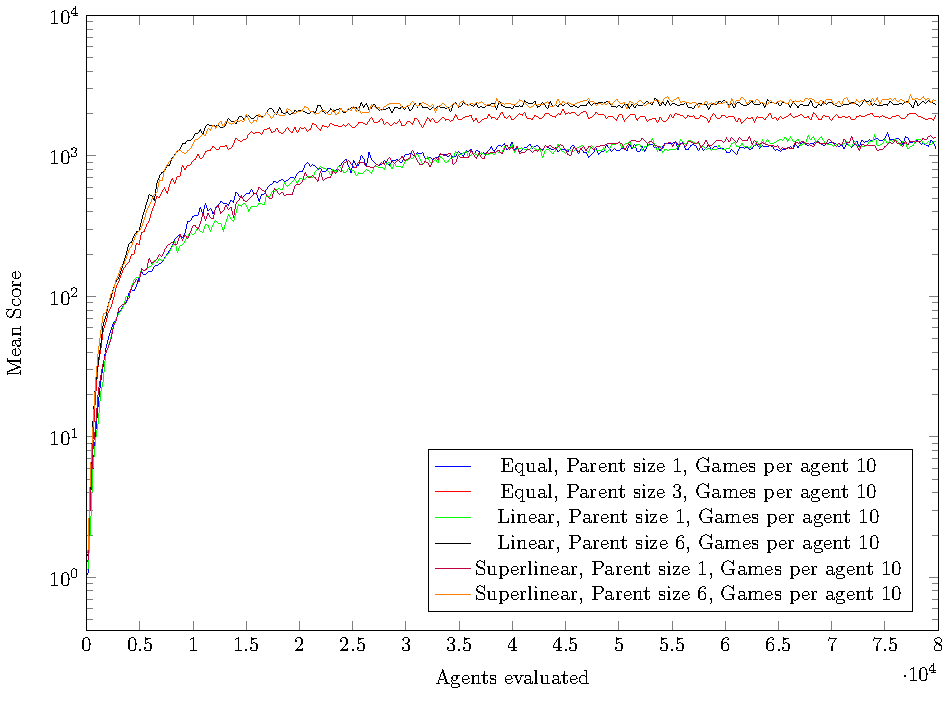
\includegraphics[scale=1]{data/cma_population_offspring/bestofeach_population/12x/PlotFile.pdf}
\caption{Best performing configurations for population size 12}
\end{figure}

\clearpage

\begin{table}[H]
\centering
\small
\begin{tabular}{c c c c r r r r}
Population & Parent & Recombination & Games per Agent & mean & Q1 & Q2 & Q3\\
\hline
$22$ & $2$ & EQUAL & 10 & $1895.305$ & $1630.891$ & $1849.75$ & $2043.442$\\
$22$ & $2$ & LINEAR & 10 & $2158.396$ & $1966.351$ & $2085.235$ & $2162.541$\\
$22$ & $2$ & SUPERLINEAR & 7 & $1783.623$ & $1603.389$ & $1720.335$ & $1937.749$\\
$22$ & $5$ & EQUAL & 10 & $2462.409$ & $2277.180$ & $2418.100$ & $2600.411$\\
$22$ & $11$ & LINEAR & 7 & $2763.353$ & $2597.450$ & $2705.080$ & $3000.242$\\
$22$ & $11$ & SUPERLINEAR & 10 & $2849.220$ & $2500.231$ & $2835.450$ & $3143.121$\\
\end{tabular}
\caption{Best performing configurations for population size 22}
\end{table}

\begin{figure}[H]
\centering
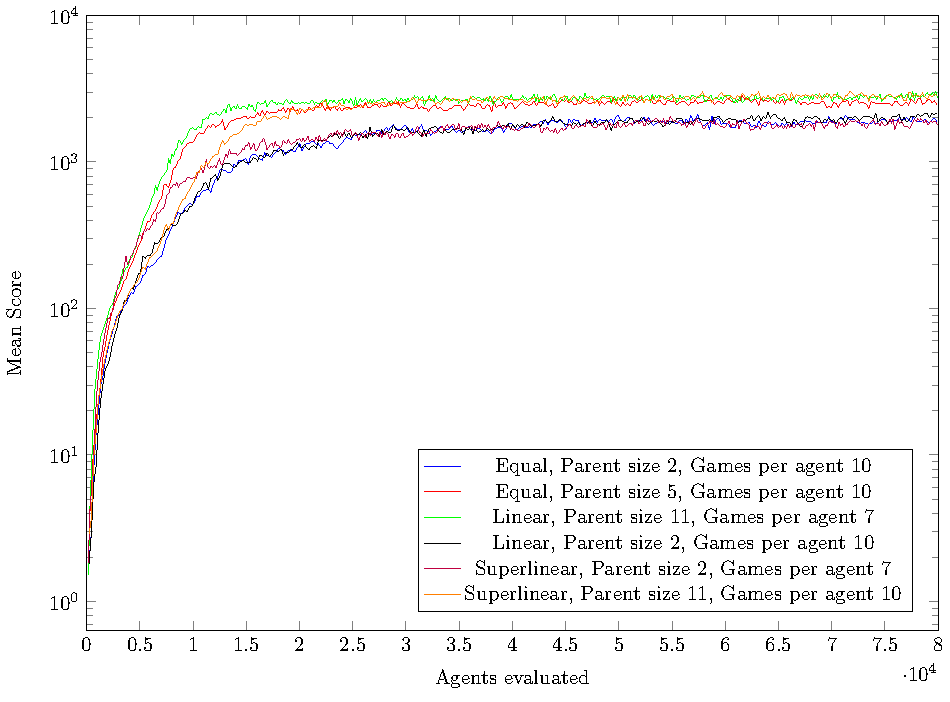
\includegraphics[scale=1]{data/cma_population_offspring/bestofeach_population/22x/PlotFile.pdf}
\caption{Best performing configurations for population size 22}
\end{figure}

\clearpage

\begin{table}[H]
\centering
\small
\begin{tabular}{c c c c r r r r}
Population & Parent & Recombination & Games per Agent & mean & Q1 & Q2 & Q3\\
\hline
$50$ & $5$ & EQUAL & 10 & $2801.923$ & $2479.088$ & $2915.980$ & $3081.018$\\
$50$ & $5$ & LINEAR & 7 & $2842.090$ & $2497.952$ & $2922.965$ & $3136.509$\\
$50$ & $5$ & SUPERLINEAR & 10 & $2757.388$ & $2357.062$ & $2886.950$ & $3187.282$\\
$50$ & $12$ & EQUAL & 10 & $2957.794$ & $2636.478$ & $2843.380$ & $3222.420$\\
$50$ & $25$ & LINEAR & 10 & $3167.873$ & $2941.590$ & $3130.385$ & $3415.520$\\
$50$ & $25$ & SUPERLINEAR & 5 & $3211.658$ & $2889.689$ & $3305.485$ & $3694.480$\\
\end{tabular}
\caption{Best performing configurations for population size 50}
\end{table}

\begin{figure}[H]
\centering
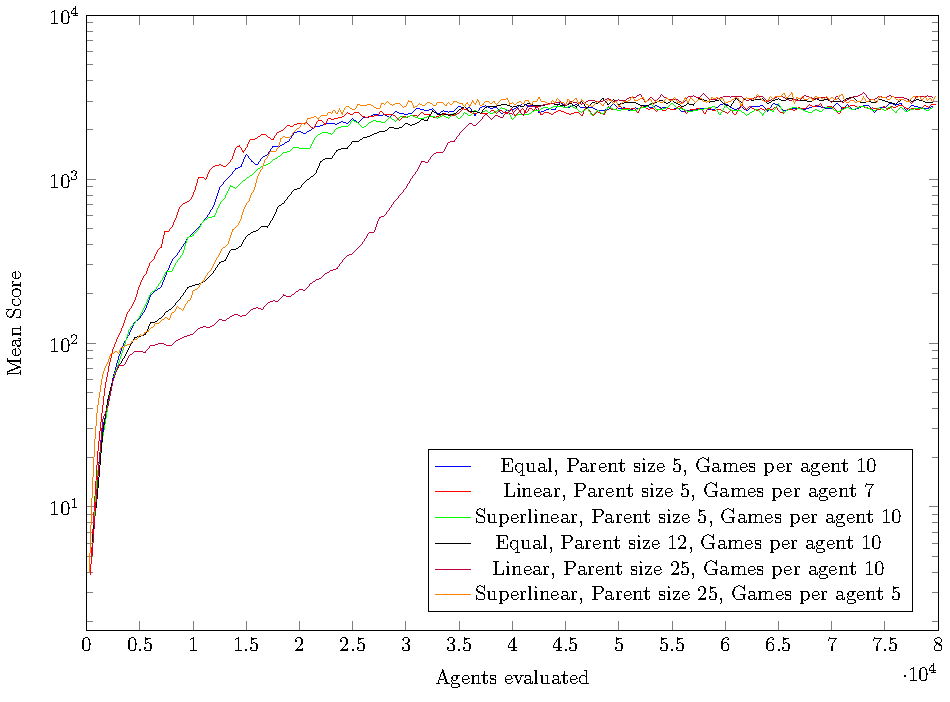
\includegraphics[scale=1]{data/cma_population_offspring/bestofeach_population/50x/PlotFile.pdf}
\caption{Best performing configurations for population size 50}
\end{figure}

\clearpage

\begin{table}[H]
\centering
\small
\begin{tabular}{c c c c r r r r}
Population & Parent & Recombination & Games per Agent & mean & Q1 & Q2 & Q3\\
\hline
$100$ & $10$ & EQUAL & 7 & $3016.342$ & $2835.049$ & $2985.150$ & $3292.910$\\
$100$ & $10$ & LINEAR & 5 & $3204.395$ & $2928.050$ & $3248.515$ & $3371.008$\\
$100$ & $10$ & SUPERLINEAR & 5 & $3009.495$ & $2816.660$ & $2989.900$ & $3189.310$\\
$100$ & $25$ & EQUAL & 3 & $3244.544$ & $2924.488$ & $3270.885$ & $3525.671$\\
$100$ & $50$ & LINEAR & 7 & $3322.076$ & $3160.098$ & $3289.370$ & $3537.850$\\
$100$ & $50$ & SUPERLINEAR & 5 & $3304.119$ & $3004.140$ & $3226.235$ & $3679.359$\\
\end{tabular}
\caption{Best performing configurations for population size 100}
\end{table}

\begin{figure}[H]
\centering
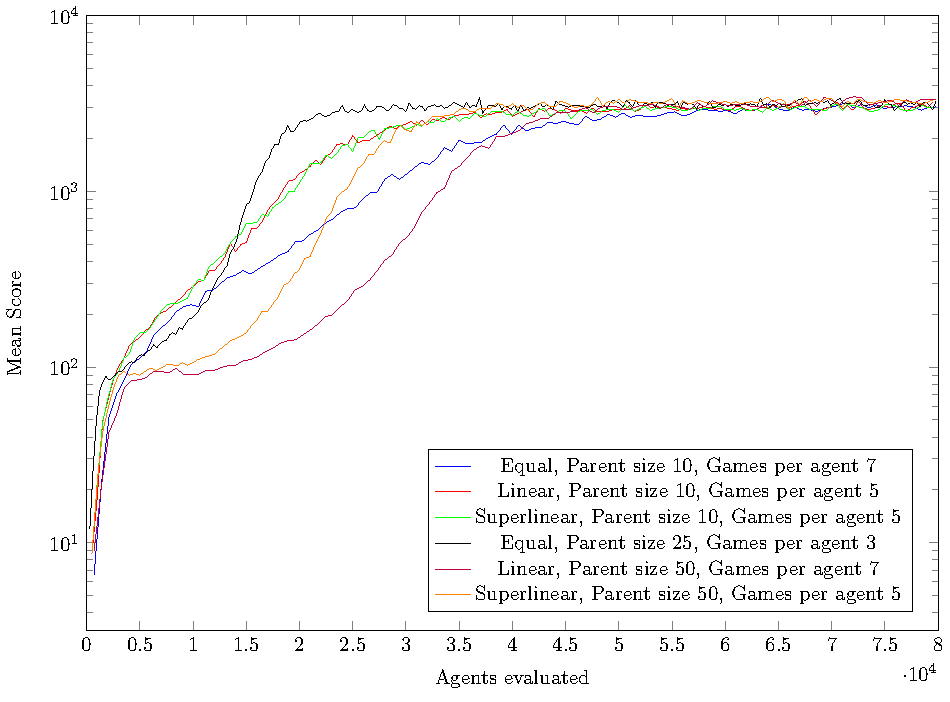
\includegraphics[scale=1]{data/cma_population_offspring/bestofeach_population/100x/PlotFile.pdf}
\caption{Best performing configurations for population size 100}
\end{figure}

\clearpage 

\begin{table}[H]
\centering
\small
\begin{tabular}{c c c c r r r r}
Population & Parent & Recombination & Games per Agent & mean & Q1 & Q2 & Q3\\
\hline
$12$ & $6$ & SUPERLINEAR & 10 & $2472.293$ & $2194.049$ & $2430.780$ & $2709.040$\\
$22$ & $11$ & SUPERLINEAR & 10 & $2849.220$ & $2500.231$ & $2835.450$ & $3143.121$\\
$50$ & $25$ & SUPERLINEAR & 5 & $3211.658$ & $2889.689$ & $3305.485$ & $3694.480$\\
$100$ & $50$ & LINEAR & 7 & $3322.076$ & $3160.098$ & $3289.370$ & $3537.850$\\
\end{tabular}
\caption{Best performing configurations of all population sizes}
\end{table}

\begin{figure}[H]
\centering
\includegraphics[scale=1]{data/cma_population_offspring/bestofall_population/PlotFile.pdf}
\caption{Best performing configurations of all population sizes}
\end{figure}



\clearpage

\subsection{Comparison - Initial comparison}
Comparison between the verified Cross Entropy and Shark (reference to shark) stock setting CMA.

\begin{table}[h]
\centering
\small
\caption{Shark stock CMA and Verified Cross Entropy}
\begin{tabular}{l r}
Optimizer & CMA\\
Number of Evaluations & 8000\\
Number of Learning Games & 30\\
Population size& 13\\
Parent size & 6\\
Games per Agent & 1\\
Tetris Type & Normal\\
\hline
Recombination Type & Superlinear\\
Initial Sigma & (what is stock)\\
\quad & \quad
\end{tabular}
\quad
\begin{tabular}{l r}
Optimizer & Cross Entropy\\
Number of Evaluations & 8000\\
Number of Learning Games & 30\\
Population size & 100\\
Parent size & 10\\
Games per Agent & 1\\
Tetris Type & Normal\\
\hline
Sigma & 100\\
Noise Type & Constant\\
Noise & 4
\end{tabular}
\end{table}

INSERT PLOTS HERE.

\clearpage

\subsection{Comparison - Comparison of featuresets}
Experiments to test Bertsekas and Dellacherie featuresets in regards to achieved score. This will tell if a different featureset affects the algorithms performance. If the behaviour is the same, then the Tetris complexity problem

\begin{table}[h]
\centering
\small
\caption{Shark stock CMA and Verified Cross Entropy}
\begin{tabular}{l r}
Optimizer & CMA\\
Number of Evaluations & 8000\\
Number of Learning Games & 30\\
Population size& 13\\
Parent size & 6\\
Games per Agent & 1\\
Tetris Type & Hard\\
\hline
Recombination Type & Superlinear\\
Initial Sigma & (what is stock)\\
\quad & \quad
\end{tabular}
\quad
\begin{tabular}{l r}
Optimizer & Cross Entropy\\
Number of Evaluations & 8000\\
Number of Learning Games & 30\\
Population size & 100\\
Parent size & 10\\
Games per Agent & 1\\
Tetris Type & Hard\\
\hline
Sigma & 100\\
Noise Type & Constant\\
Noise & 4
\end{tabular}
\end{table}

Used on the bertsekas and Dellacherie featuresets

INSERT PLOTS HERE.

\section{CMA initial step-size}

Shows the graps of the configuration test, with initial sigma
settings.

 - \comment{Insert in above section}

\section{Cross Entropy configuration settings \label{appendixCrossEntropyConfig}}

The plots from the configuration of cross entropy.
All plots shows the numbers of games played along the x-axis
and the mean score of the centroid agent along the y-axis.

\begin{tabular}{@{}l@{}l@{}}
\includegraphics[scale=1]{plots/ce_ConstantNoise_l10_o1_all} &
\includegraphics[scale=1]{plots/ce_ConstantNoise_l13_o6_all} //
\includegraphics[scale=1]{plots/ce_ConstantNoise_l10_o5_all} &
\end{tabular}

\begin{tabular}{@{}l@{}l@{}}
\includegraphics[scale=1]{plots/ce_ConstantNoise_l22_o2_all}&
\includegraphics[scale=1]{plots/ce_ConstantNoise_l22_o2_all}
\end{tabular}

\begin{tabular}{@{}l@{}l@{}}
\includegraphics[scale=1]{plots/ce_ConstantNoise_l50_o5_all} &
\includegraphics[scale=1]{plots/ce_ConstantNoise_l50_o25_all}
\end{tabular}

\begin{tabular}{@{}l@{}l@{}}
\includegraphics[scale=1]{plots/ce_ConstantNoise_l100_o10_all} &
\includegraphics[scale=1]{plots/ce_ConstantNoise_l100_o50_all}
\end{tabular}

\begin{tabular}{@{}l@{}l@{}}
\includegraphics[scale=1]{plots/ce_ConstantNoise_l200_o20_all} &
\includegraphics[scale=1]{plots/ce_ConstantNoise_l200_o100_all}
\end{tabular}





 - \comment{Insert in above section}

\clearpage

\section{Cross Entropy Implementation - Shark library}

\subsection{CrossEntropyMethod.h}

\lstinputlisting[language=c++, style=customc]{CrossEntropyMethod.h}

\clearpage

\subsection{CrossEntropyMethod.cpp}

\lstinputlisting[language=c++, style=customc]{CrossEntropyMethod.cpp}
